\documentclass[11pt]{report}
\usepackage{styles/chuck_manual}

\begin{document}

%%%%%%%%%%%%%%%%%%%%% TITLE PAGE
% this is a little too hacky..... but it works
\thispagestyle{coverplain}
\vskip 6in
{\huge

\makebox[\textwidth][s]{{\underline{T} h e \underline{C} h u c K \underline{M} a n u a l}}

}

\vskip 2in
\begin{center}
  
\includegraphics[height=4in]{images/chuck_logo2.jpg}

  \vskip 1in

  \Large{\href{http://chuck.cs.princeton.edu/}{http://chuck.cs.princeton.edu/}}
\end{center}

\newpage

%%%%%%%%%%%%%%%%%%%%  OPENING MATTER
%\colorbox{lightgray}{\parbox{\textwidth}{here is may text which goes over many lines}}

\pagenumbering{roman}

\newpage
\section{Authors of ChucK}

Originated by:\\
\authtab Ge Wang\\
\authtab Perry R. Cook\\

Chief Architect and Design:\\
\authtab Ge Wang\\

Lead Developers:\\
\authtab Ge Wang -- gewang@cs.princeton.edu $|$ ge@ccrma.stanford.edu\\
\authtab Perry R. Cook -- prc@cs.princeton.edu\\
\authtab Ananya Misra -- amisra@cs.princeton.edu\\
\authtab Spencer Salazar -- ssalazar@cs.princeton.edu\\
\authtab Rebecca Fiebrink -- fiebrink@cs.princeton.edu\\
\authtab Philip Davidson -- philipd@alumni.princeton.edu\\
\authtab Ari Lazier -- alazier@cs.princeton.edu\\

Documentation:\\
\authtab Adam Tindale -- adam.tindale@acad.ca\\
\authtab Ge Wang\\
\authtab Rebecca Fiebrink\\
\authtab Philip Davidson\\
\authtab Ananya Misra\\
\authtab Spencer Salazar\\

Lead Testers:\\
\authtab The ChucK Development/User Community -- http://chuck.cs.princeton.edu/community/\\
\authtab Ge Wang\\
\authtab Philip Davidson\\
\authtab Ajay Kapur -- akapur@alumni.princeton.edu\\


Many people have further contributed to ChucK by suggesting great new ideas and improvements, reporting problems, or submitting actual code. Here is a list of these people.  Help us keep it complete and exempt of errors.

\begin{chuckitemize}
\item Andrew Appel 
\item Brian Kernighan 
\item Paul Lansky 
\item Roger Dannenberg
\item Dan Trueman 
\item Ken Steiglitz 
\item Max Mathews
\item Szymon Rusinkiewicz 
\item Graham Coleman
\item Scott Smallwood
\item Mark Daly
\item Kassen
\item Kijjaz
\item Gary Scavone 
\item Brad Garton
\item Nick Collins 
\item Tom Briggs 
\item Paul Calamia 
\item Mikael Johanssons 
\item Magnus Danielson 
\item Rasmus Kaj 
\item Princeton Graphics Group
\item Princeton Laptop Orchestra
\item Stanford Laptop Orchestra
\item ChucK users community!!!
\end{chuckitemize}


\newpage
\section{ChucK Places}


ChucK home page:\\
\urltab    \href{http://chuck.cs.princeton.edu/}{http://chuck.cs.princeton.edu/}

Princeton Sound Lab:\\
\urltab    \href{http://soundlab.cs.princeton.edu/}{http://soundlab.cs.princeton.edu/}  
    
ChucK Documentation + Tutorials:\\
\urltab    \href{http://chuck.cs.princeton.edu/doc/}{http://chuck.cs.princeton.edu/doc/}
    
For the most updated tutorial:\\
\urltab    \href{http://chuck.cs.princeton.edu/doc/learn/}{http://chuck.cs.princeton.edu/doc/learn/}
    
For the ideas and design behind ChucK, read the papers at:\\
\urltab    \href{http://chuck.cs.princeton.edu/doc/publish/}{http://chuck.cs.princeton.edu/doc/publish/}
    
ChucK Developer's Guide:\\
\urltab    \href{http://chuck.cs.princeton.edu/doc/develop/}{http://chuck.cs.princeton.edu/doc/develop/}

ChucK WIKI\\
\urltab    \href{http://chuck.cs.princeton.edu/wiki}{http://chuck.cs.princeton.edu/wiki}

\tableofcontents
\clearpage

%%%%%%%%%%%%%%%%%%%%  MAIN MATTER
\pagestyle{fancy}

\part*{Getting Started}

\pagenumbering{arabic}

\chapter{Intro-ChucK-tion} 

{\bf what is it:} ChucK is a general-purpose programming language, intended for 
real-time audio synthesis and graphics/multimedia programming.  It 
introduces a truly concurrent programming model that embeds timing 
directly in the program flow.  Other potentially useful features include 
the ability to write/change programs on-the-fly.

{\bf who it is for:} audio/multimedia researchers, developers, composers, and performers

\underline{supported platforms:}
\begin{itemize}
 \item MacOS X (CoreAudio)
 \item Linux (ALSA/OSS/Jack)
 \item Windows/Cygwin (DirectSound)
 \item SGI (coming soon)
\end{itemize}

\section*{On-the-fly Programming}
On-the-fly programming is a style of programming in which the programmer/performer/composer 
augments and modifies the program while it is running, without stopping or restarting, 
in order to assert expressive, programmable control for performance, composition, and 
experimentation at run-time. Because of the fundamental powers of programming languages, 
we believe the technical and aesthetic aspects of on-the-fly programming are worth exploring.

\chapter{Installation}

We tried to make ChucK as easy as possible to build and re-use. All 
sources files - headers source for compiler, vm, and audio engine - are 
in the same directory (they run in the same address space anyway). Platforms 
differences are abstracted to the lowest level (in part thanks to Gary 
Scavone). None of the compiler/vm has any OS-depedent code.

There are also pre-compiled executables available for OS X and Windows.

\section{Binary Installation}

The binary distributions include a directory called bin/ that contains the precompiled binary of ChucK for your operating system. The binary distribution is a great introduction to ChucK but once you are comfortable we suggest that you compile ChucK on your own system so that it is optimized for your system. 

\subsection{OS X}
1. The terminal is located in the Utilities/ folder in the Applications/ folder of your hard drive. In the terminal go to the bin/ directory (replace chuck-x.x.x.x-exe with the actual directory name):

\chuckterm{
   \prompt cd chuck-x.x.x.x-exe/bin
}

2. Install it using the script included.

\chuckterm{
    \prompt sudo cp chuck /usr/bin/
}

(enter password when prompted)

\chuckterm{    
    \prompt sudo chmod 755 /usr/bin/chuck
}

Now you should be able to run 'chuck' from any directory.

3. Test to make sure it is was installed properly.

\chuckterm{
    \prompt chuck
}

You should see the following message (which is the correct behavior):

\chuckterm{
    [chuck]: no input files... (try --help)
}


\subsection{Windows}

1. Place chuck.exe (found in the 'bin' folder) into c:\textbackslash windowss\textbackslash system32\textbackslash

2. Open a command window found in start-\textgreater run

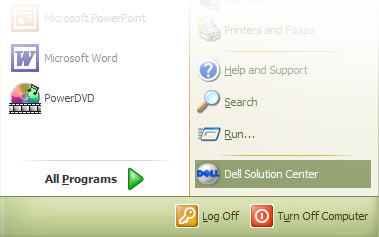
\includegraphics{images/startmenu}

3. Type cmd and press return

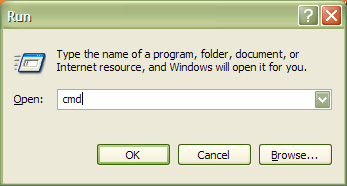
\includegraphics{images/cmd}

4. Type chuck and press return, you should see:

\chuckterm{
    \prompt chuck
    
    [chuck]: no input files... (try --help)
}

\section{Source Installation}

To build chuck from the source (from scratch): 

1. Go to the src/ directory (replace chuck-x.x.x.x with the actual 
directory name):

\chuckterm{
   \prompt cd chuck-x.x.x.x/src/
}


2. If you type 'make' here, you should get the following message:

\chuckterm{
   \prompt make\\
   \chuckbuild: please use one of the following configurations:\\
       make osx, make osx-intel, make linux-oss, make linux-alsa, make linux-jack, make win32
}

Now, type the command corresponding to your platform... 

for example, for MacOS X:

\chuckterm{\prompt make osx}

for example, for Windows:

\chuckterm{\prompt make win32}

3. If you would like to install chuck (cp into /usr/bin by default). If you 
don't like the destination, simply edit the makefile under `install', or 
skip this step altogether. (we recommend putting it somewhere in your 
path, it makes on-the-fly programming easier)

\chuckterm{
   \# (optional: edit the makefile first)\\
   \prompt make install
}

You may need to have administrator privileges in order to install ChucK. If you 
have admin access then you can use the sudo command to install.

\chuckterm{
   \prompt sudo make install
}

4. If you haven't gotten any egregious error messages up to this point, 
then you should be done! There should be a `chuck' executable in the 
current directory. For a quick sanity check, execute the following (use 
`./chuck' if chuck is not in your path), and see if you get the same output:

\chuckterm{
   \prompt chuck
   [chuck]: no input files...
}

(if you do get error messages during compilation, or you run into some 
other problem - please let us know and we will do our best to provide 
support) 

\rule{1in}{.5pt}

You are ready to ChucK. If this is your first time programming in 
ChucK, you may want to look at the documentation, or take the ChucK 
Tutorial ( \href{http://chuck.cs.princeton.edu/doc}{http://chuck.cs.princeton.edu/doc/}). 

ThanK you very much. Go forth and ChucK - email us for support or to make a 
suggestion or to call us idiots.

Ge + Perry
 


%%% tutorials
  \chapter{ChucK Tutorials}

\section{A Chuck Tutorial}
Hello ChucK: 

\textit{This tutorial was written for the command line version of ChucK (currently the most stable and widely supported).  Other ways of running ChucK include using the miniAudicle (download and documentation at: \href{http://audicle.cs.princeton.edu/mini/}{http://audicle.cs.princeton.edu/mini/}) and the Audicle (in pre-pre-alpha).  The ChucK code is the same, but the way to run them differs, depending the ChucK system.}

The first thing we are going to do is do generate a sine wave and send it to the speaker so we can hear it. We can do this easily in ChucK by connecting audio processing modules (unit generators) and having them work together to compute the sound. 

We start with a blank ChucK program and add the following line of code:
\begin{verbatim}
        // connect sine oscillator to D/A convertor (sound card)
        SinOsc s => dac;
\end{verbatim}

NOTE: by default, a ChucK program starts executing from the first instruction in the top-level (global) scope.

The above does several things:
\begin{enumerate}
\item it creates a new unit generator of type `SinOsc' (sine oscillator), and stores its reference in variable `s'.
\item `dac' (D/A convertor) is a special unit generator (created by the system) which is our abstraction for the underlying audio interface.
\item we are using the ChucK operator (\chuckop) to ChucK `s' to `dac'. In ChucK, when one unit generator is ChucKed to another, we connect them. We can think of this line as setting up a data flow from `s', a signal generator, to `dac', the sound card/speaker. Collectively, we will call this a `patch'. 
\end{enumerate}

The above is a valid ChucK program, but all it does so far is make the connection -- if we ran this program, it would exit immediately. In order for this to do what we want, we need to take care of one more very important thing: time. Unlike many other languages, we don't have to explicitly say ``play'' to hear the result. In ChucK, we simply have to ``allow time to pass'' for data to be computed. As we will see, time and audio data are both inextricably related in ChucK (as in reality), and separated in the way they are manipulated. But for now, let's generate our sine wave and hear it by adding one more line:

\begin{verbatim}
        // connect sine oscillator to D/A convertor (sound card)
        SinOsc s => dac;

        // allow 2 seconds to pass
        2::second => now;
\end{verbatim}

Let's now run this (assuming you saved the file as `foo.ck'):

\chuckterm{\prompt chuck foo.ck}

This would cause the sound to play for 2 seconds (the :: operator simply multiplies the arguments), during which time audio data is processed (and heard), after which the program exits (since it has reached the end). For now, we can just take the second line of code to mean ``let time pass for 2 seconds (and let audio compute during that time)''. If you want to play it indefinitely, we could write a loop:

\begin{verbatim}
        // connect sine oscillator to D/A convertor (sound card)
        SinOsc s => dac;

        // loop in time
        while( true ) {
            2::second => now;
        }
\end{verbatim}

In ChucK, this is called a `time-loop' (in fact this particular one is an `infinite time loop'). This program executes (and generate/process audio) indefinitely. Try running this program. 

\paragraph*{IMPORTANT:} perhaps more important than how to run ChucK is how to \textit{stop} ChucK.  To stop a ongoing ChucK program from the command line, hit (ctrl \- c).

So far, since all we are doing is advancing time; it doesn't really matter (for now) what value we advance time by - (we used 2::second here, but we could have used any number of `ms', `second', `minute', `hour', `day', and even `week'), and the result would be the same. It is good to keep in mind from this example that almost everything in ChucK happens naturally from the timing. 

Now, let's try changing the frequency randomly every 100ms:
\begin{verbatim}

        // make our patch
        SinOsc s => dac;

        // time-loop, in which the Osc's frequency is changed every 100 ms
        while( true ) {
            100::ms => now;
            Std.rand2f(30.0, 1000.0) => s.freq;
        }
\end{verbatim}

This should sound like computer mainframes in old sci-fi movies. Two more things to note here. (1) We are advancing time inside the loop by 100::ms durations. (2) A random value between 30.0 and 1000.0 is generated and 'assigned' to the oscillator's frequency, every 100::ms. 

Go ahead and run this (again replace foo.ck with your filename):
\chuckterm{\prompt chuck foo.ck}

Play with the parameters in the program. Change 100::ms to something else (like 50::ms or 500::ms, or 1::ms, or 1::samp\textit{(every sample)}), or change 1000.0 to 5000.0. 

Run and listen:
\chuckterm{\prompt chuck foo.ck}

Once things work, hold on to this file - we will use it again soon. 

Concurrency in ChucK: 

Now let's write another (slightly longer) program:
\begin{verbatim}
        // impulse to filter to dac
        Impulse i => BiQuad f => dac;
        // set the filter's pole radius
        .99 => f.prad;
        // set equal gain zero's
        1 => f.eqzs;
        // initialize float variable
        0.0 => float v;

        // infinite time-loop
        while( true )
        {
            // set the current sample/impulse
            1.0 => i.next;
            // sweep the filter resonant frequency
            Std.fabs(Math.sin(v)) * 4000.0 => f.pfreq;
            // increment v
            v + .1 => v;
            // advance time
            100::ms => now;
        }
\end{verbatim}

Name this moe.ck, and run it:
\chuckterm{\prompt chuck moe.ck}

Now, make two copies of moe.ck - larry.ck and curly.ck. Make the following modifications:
\begin{enumerate}
\item change larry.ck to advance time by 99::ms (instead of 100::ms).
\item change curly.ck to advance time by 101::ms (instead of 100::ms). 
\item optionally, change the 4000.0 to something else (like 400.0 for curly). 
\end{enumerate}

Run all three in parallel:
\chuckterm{\prompt chuck moe.ck larry.ck curly.ck}

What you hear (if all goes well) should be 'phasing' between moe, larry, and curly, 
with curly emitting the lower-frequency pulses. 

ChucK supports sample-synchronous concurrency via the ChucK timing mechanism. Given any 
number of source files that uses the timing mechanism above, the ChucK VM can use the timing 
information to automatically synchronize all of them. Furthermore, the concurrency is 
'sample-synchronous', meaning that inter-process audio timing is guaranteed to be precise to 
the sample. The audio samples generated by our three stooges in this examples are completely 
synchronized. Note that each process do not need to know about each other - it only has to deal 
with time locally. The VM will make sure things happen correctly and globally. 

  \section{Conventions}

ChucK is supported under many different operating systems. While ChucK code is intended to be truly "platform-independent", each different OS has their own ``features'' that make the experience of working with ChucK slightly different. This chapter will outline some of these differences. 

%(no, ChucK is not sick, but it may cause nausea, stress, frustration...). 
ChucK is used as a terminal application in this tutorial, so you will need to know how to access and navigate in the terminal. Here are some hints about getting started with the terminal on your operating system.


\subsection{OS X}

The terminal is located in the Utilities/ folder in the Applications/ folder of your hard drive. Double click on Terminal. You can click and hold on the icon in the Dock and select the ``Keep in Dock'' option. Now the Terminal application will be conveniently located in the Dock. 

\href{http://www.macdevcenter.com/pub/ct/51}{http://www.macdevcenter.com/pub/ct/51}

\href{http://www.atomiclearning.com/macosxterminalx.shtml}{http://www.atomiclearning.com/macosxterminalx.shtml}

\subsection{Windows}

The terminal is accessed by clicking on the Start Menu and then clicking on run. In the window that opens type {\bf cmd}. 

\href{http://www.c3scripts.com/tutorials/msdos/}{http://www.c3scripts.com/tutorials/msdos/}

\href{http://www.ss64.com/nt/}{http://www.ss64.com/nt/}

\subsection{Linux}

No hints needed here.
% If you are reading this then you are required to return your tinfoil hat.

  \section{On-the-fly-programming}
\textbf{by Adam Tindale}\\

Navigate to the examples folder in the ChucK distribution then run the following command:

\chuckterm{\prompt chuck moe.ck}

In this case, ChucK will run whatever is in {\bf moe.ck}. You can replace {\bf moe.ck} with the name of another ChucK file. If this script is a just a loop that never ends then we need to stop ChucK eventually. Simply press CTRL-C (hold control and press c). This is the "kill process" hotkey in the terminal. 

Some first things to try is to test the concurrency (running multiple ChucK files in parallel) are moe, larry, and curly. First, run them each individually ( run chuck on {\bf moe.ck}, {\bf larry.ck}, or {\bf curly.ck} as shown above).  Then, run them all in parallel, like this:

\chuckterm{\prompt chuck moe.ck larry.ck curly.ck}

They are written to go in and out of phase with each other.  Again, if any of these scripts will go on forever then you have to use CTRL-C to halt ChucK. 
%Why would you do that? If the script has some random number generators or something like that then you end up with some nice ChucK chaos not just copies of the same patch! 
Give it a try. 

Also try the improved versions of our little friends: {\bf larry++.ck curly++.ck moe++.ck} 

\section*{Two Window ChucK}
Now lets roll up our sleeves a little bit and see some real ChucK power! We are going to run two window ChucK, and on-the-fly! This section will walk you through a ChucK session. 

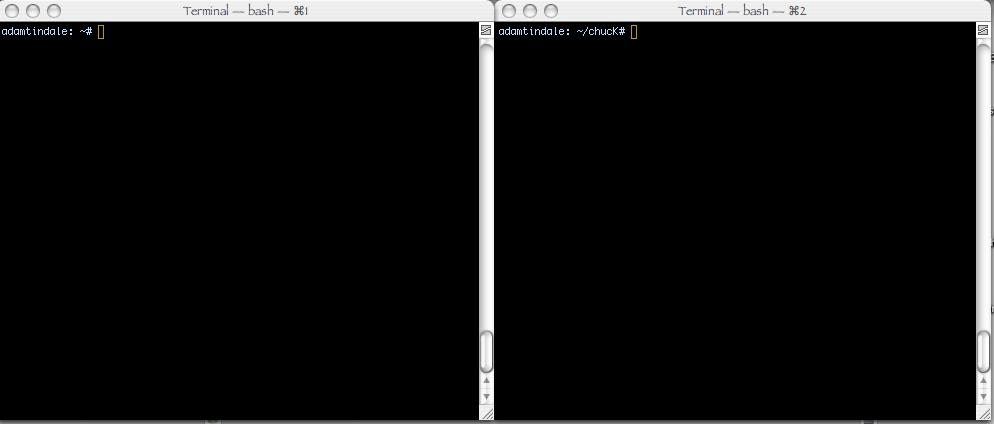
\includegraphics[width=\textwidth]{images/2term}

Here is what you do: open another terminal window just like this one. In this new window type:
\chuckterm{\prompt chuck \doubledash loop}

This will start ChucK running. ChucK is now waiting for something to do. Go back to your original window where you are in your ChucK home. Be careful. If you type chuck test1.ck you will start a second ChucK running test1.ck. What we want to do is add a script to the ChucK that we set running in our second window. We will use the + operator to add a script to our ChucK and the - operator to remove a script. 

\chuckterm{\prompt chuck + test1.ck\\
  \prompt chuck - 1\\
  \prompt chuck test.ck\\
  \prompt chuck test.ck\\
  \prompt chuck test.ck
}

What happened? That is the power of on-the-fly programming. We added test1.ck. It was added as the first shred in our ChucK. Since we knew it was shred 1 we removed it by typing chuck - 1. Great. Next we added three copies of the same script! Isn't that cool? You can also do this chuck + test1.ck test1.ck test1.ck How do you keep track of shreds? 

You can ask ChucK how he is doing by typing chuck \doubledash status The shortcut is chuck \^ ChucK will answer in the other window where we left him running. He will tell you what shreds there are and what their id numbers are. He will also tell you how long he has been running. 

When you have had enough of ChucK you can go to the other window and use your fancy CTRL-C trick or you can type chuck \doubledash kill in your original window.   

\chuckterm{\prompt chuck \doubledash kill}

\section*{One Window ChucK}

So you think you are pretty good? One window ChucK is only for the hardest of hardcore.\footnote{As one adventurous Windows user has noted, due to its reliance on launching background processes, it is in fact only for the hardest of hardcore Mac and Linux users, or those valiant Windows traitors employing Cygwin or similar Unix-like interfaces.} You have been warned. 

The concept is pretty similar to two window ChucK: first, you start a ChucK going, then you manage the adding and removal of scripts to it. How do you start a ChucK and get the command prompt to return, you ask? In your shell you can add an ampersand (\& ) after the command and that will tell the shell to run the command as a background process and give you the prompt back. 

\chuckterm{\prompt chuck \doubledash loop \& }

The rest is as it should be. You will have to be careful when writing your patches to not put too many print statements. When you print you will temporarily lose control of the prompt as the shell prints. This can be bad when are you are printing MIDI input. The same applies when you use the \doubledash status command to ChucK. It can also be fun to fight for your command line. Who will win?

  % OLD STUFF -- duplicated by "chuck_tutorial.tex"
\section{Writing Your First Patch}

The first thing we are going to do is do generate a sine wave and send to the speaker so we can hear it. We can do this easily ChucK by connecting audio processing modules (unit generators) and having them work together to compute the sound. 

We start with a blank ChucK program, and add the following line of code: (by default, a ChucK program starts executing from the first instruction in the top-level (global) scope).
\begin{verbatim}
        // connect sine oscillator to D/A convertor (sound card)
        sinosc s => dac;
\end{verbatim}

The above does several things: 

(1) it creates a new unit generator of type `sinosc' (sine oscillator), and store its reference in variable `s'. 

(2) `dac' (D/A convertor) is a special unit generator (created by the system) which is our abstraction for the underlying audio interface. 

(3) we are using the ChucK operator (\chuckop) to ChucK `s' to `dac'. In ChucK, when one unit generator is ChucKed to another, we connect them. We can think of this line as setting up a data flow from `s', a signal generator, to `dac', the sound card/speaker. 

Collectively, we will call this a `patch'. 

The above is a valid ChucK program, but all it does so far is make the connection (if we ran this program, it would exit immediately). In order for this to do what we want, we need to take care of one more very important thing: time. Unlike many other languages, we don't have to explicitly say "play" to hear the result. In ChucK, we simply have to ``allow time to pass'' for data to be computed. As we will see, time and audio data are both inextricably related in ChucK (as in reality), and separated in the way they are manipulated. But for now, let's generate our sine wave and hear it by adding one more line:

\begin{verbatim}
        // connect sine oscillator to D/A convertor (sound card)
        sinosc s => dac;

        // allow 2 seconds to pass
        2::second => now;
\end{verbatim}

Let's now run this (assuming you saved the file as `foo.ck'):

\chuckterm{\prompt chuck foo.ck}

This would cause the sound to play for 2 seconds, during which time audio data is processed (and heard), after which the program exits (since it has reached the end). For now, we can just take the second line of code to mean ``let time pass for 2 seconds (and let audio compute during that time)''. If you want to play it indefinitely, we could write a loop:

\begin{verbatim}
        // connect sine oscillator to D/A convertor (sound card)
        sinosc s => dac;

        // loop in time
        while( true ) {
            2::second => now;
        }
\end{verbatim}

In ChucK, this is called a `time-loop' (in fact this is an `infinite time loop'). This program executes (and generate/process audio) indefinitely. Try runnig this program. (Remember CONTROL-C can kill ChucK when you get sick of this patch.)

So far, since all we are doing is advancing time, it doesn't really matter (for now) what value we advance time by - (we used 2::second here, but we could have used any number of `ms', `second', `minute', `hour', `day', and even `week'), and the result would be the same. It is good to keep in mind from this example that almost everything in ChucK happens naturally from the timing. 

Now, let's try changing the frequency randomly every 100ms:
\begin{verbatim}

        // make our patch
        sinosc s => dac;

        // time-loop, in which the osc's frequency is changed every 100 ms
        while( true ) {
            100::ms => now;
            std.rand2f(30.0, 1000.0) => s.freq;
        }
\end{verbatim}

This should sound like computer mainframes in old sci-fi movies. Two more things to note here. 

(1) We are advancing time inside the loop by 100::ms durations. 

(2) A random value between 0.0 and 800.0 is generated and 'assigned' to the oscillator's frequency, every 100::ms. 

Go ahead and run this (again replace foo.ck with your filename):
\chuckterm{\prompt chuck foo.ck}

Play with the parameters in the program. Change 100::ms to something else (like 50::ms or 500::ms), or change 400.0 to 4000.0. Experiment and have fun!

  \section{Modifying Basic Patches}

We have a basic patch running in ChucK but it still doesn't sound very good. In this chapter we will cover some simple ways to rectify that problem. ChucK allows one to quickly make modifications to patches that can drastically change the sound.

First what we can do is change the type of our oscillator. There are many different oscillators available to use: sinosc (sine wave), sawosc (sawtooth), sqrosc (square wave) and  pulseosc (pulse wave). We can simply change the type of oscillator just like below. 

\begin{verbatim}
        sawosc s => dac;
\end{verbatim}

Try changing the oscillator to all of the different types and a get a feel for how they sound. When changing the different Ugens always be sure to check the rest of your patches so that the parameter calls are valid. If you were to use the {\bf .width} method of pulseosc and others on a sinosc ChucK will complain. You can comment out lines that are temporarily broken by using double slashes (//).

Now let's add some effects to our patch. ChucK has many different standard effects that can be added to Ugen chains. The simplest effect we can add is an amplifier. In ChucK, this object is {\bf gain}.

\begin{verbatim}
        sawosc s => gain g => dac;
\end{verbatim}

Now we can change the parameters of our effect. {\bf gain} has a parameter {\bf .gain} that can be used to change the gain  of signals passing through the object. Let's go about changing the gain.

\begin{verbatim}
	.5 => g.gain;
\end{verbatim}

This is redundant. All Ugens have the ability to change their gain in a similar manner. 

\begin{verbatim}
	.5 => s.gain;
\end{verbatim}

However, this is useful when we have multiple Ugens connect to one place. If we were to connect 2 oscillators to the {\bf dac} then we will get distortion. By default, these oscillators oscillate between -1 and 1. When they are connected to the same input they are added, so now they go between -2 and 2. This will clip our output. What to do? {\bf gain} to the rescue!

\begin{verbatim}
	sinosc s1 => gain g => dac;
	sinsocs s2 => g;
	.5 => g.gain;
\end{verbatim}

Now our oscillators are scaled between -1 and 1 and everything is right in the world.

\subsection{Having More Fun}

More effects were promised, now you will see some in action. Again, one of the wonders of ChucK is how easy it is to change Ugens. 
  \section{LFOs and Blackhole}

A common technique to add variation to synthesis is modulation. Modulation is the process of changing someting, usually the parameter of a signal like frequency. A Low Frequency Oscillator (LFO) is typically used for this task because the variations are fast enough to be interesting, yet slow enough to be perceptable. When a signal is modulated quickly (ie. over 20Hz or so) it tends to alter the timbre of the signal rather than add variation. 

Ok, let's use this idea. What we need to do is set up two oscillators and have one modulate a paremeter of another. ChucK does not support the connection of Ugen signal outputs to parameter inputs. This piece of code will not work:

\begin{verbatim}
        sinosc s => dac;
        sinosc lfo => s.freq;
\end{verbatim}

Foiled. What we need to do is poll our lfo at some rate that we decide on, for now we will update the frequency of s every 20 milliseconds. Remember that a sinosc oscillates between -1 and 1, so if we just put that directly to the frequency of s we wouldn't be able to hear it (unless you are using ChucK in a tricked out civic...). What we are going to do is multiply the output of the lfo by 10 and add it to the frequency 440. The frequency will now oscillate between 430 and 450. 

\begin{verbatim}
        sinosc s => dac;
        sinosc lfo;

        // set the frequency of the lfo
        5 => lfo.freq;
    
        while (20::ms => now){
          ( lfo.last() * 10 ) + 440 => s.freq;
        }
\end{verbatim}

ChucK is a smart little devil. This didn't work and now we will look into the reason. Why? Ugens are connected in a network and usually passed to the {\bf dac}. When a patch is compiled ChucK looks at what is connected to the {\bf dac} and as each sample is computed ChucK looks through the network of Ugens and grabs the next sample. In this case, we don't want our Ugen connected to the {\bf dac}, yet we want ChucK to grab samples from it. Enter blackhole: the sample sucker. If we connect our lfo to blackhole everything will work out just fine.

\begin{verbatim}
        sinosc lfo => blackhole;
\end{verbatim}

Play around with this patch in its current form and find interesting values for the poll rate, lfo frequency and the lfo amount. Try changing the Ugens around for more interesting sounds as well. 


  \section{Adding Midi}

  %\section{Beats}

  %\include{chapters/chuck_tutorial_scope}
  \section{Writing To Disk}

Here is a brief tutorial on writing to disk...

---
1. recording your ChucK session to file is easy!

example:  you want to record the following:

\chuckterm{\prompt chuck foo.ck bar.ck}

all you's got to do is ChucK a shred that writes to file:

\chuckterm{\prompt chuck foo.ck bar.ck rec.ck}

no changes to existing files are necessary.
an example rec.ck can be found in examples/, this
guy/gal writes to ``foo.wav''.  edit the file to change.
if you don't want to worry about overwriting the same
file everytime, you can:

\chuckterm{\prompt chuck foo.ck bar.ck rec2.ck}

rec2.ck will generate a file name using the current
time.  You can change the prefix of the filename by
\begin{verbatim}
        "data/session" => w.autoPrefix;
\end{verbatim}
w is the WvOut in the patch.

Oh yeah, you can of course chuck the rec.ck on-the-fly...

from terminal 1
\chuckterm{\prompt chuck -\,-loop}

from terminal 2
\chuckterm{\prompt chuck + rec.ck}


---
2. silent mode

you can write directly to disk without having real-time audio
by using -\,-silent or -s

\chuckterm{\prompt chuck foo.ck bar.ck rec2.ck -s}

this will not synchronize to the audio card, and will generate
samples as fast as it can.


---
3. start and stop

you can start and stop the writing to file by:
\begin{verbatim}
        1 => w.record;  // start
        0 => w.record;  // stop
\end{verbatim}
as with all thing ChucKian, this can be done
sample-synchronously.


---
4. another halting problem

what if I have infinite time loop, and want to terminate
the VM, will my file be written out correctly?  the answer:

Ctrl-C works just fine.

ChucK STK module keeps track of open file handles and
closes them even upon abnormal termination, like Ctrl-C.
Actually for many, Ctrl-C is the natural way to end your
ChucK session.  At any rate, this is quite ghetto, but it works.
As for seg-faults and other catastrophic events, like computer
catching on fire from ChucK exploding, the file probably is
toast.

hmmmm, toast...


---
5. the silent sample sucker strikes again

as in rec.ck, one patch to write to file is:
\begin{verbatim}
        dac => gain g => WvOut w => blackhole;
\end{verbatim}
the blackhole drives the WvOut, which in turns sucks
samples from gain and then the dac.  The WvOut
can also be placed before the dac:
\begin{verbatim}
        noise n => WvOut w => dac;
\end{verbatim}
The WvOut writes to file, and also pass through the incoming samples.


  \section{Stereo}
\textbf{by Adam Tindale}\\

At long last, ChucK is stereo! Accessing the stereo capabilities of ChucK is relatively simple. {\bf dac} now has three access points. 

\begin{verbatim}
    UGen u;
    // standard mono connection
    u => dac;

    // simple enough!
    u => dac.left;
    u => dac.right;
\end{verbatim}

{\bf adc} functionality mirrors dac. 

\begin{verbatim}
    // switcheroo
    adc.right => dac.left;
    adc.left => dac.right;
\end{verbatim}

If you have your great UGen network going and you want to throw it somewhere in the stereo field you can use {\bf Pan2}. You can use the {\bf .pan} function to move your sound between left (-1) and right (1).

\begin{verbatim}
    // this is  a stereo connection to the dac
    SinOsc s => Pan2 p => dac;
    1 => p.pan;
    while(1::second => now){
        // this will flip the pan from left to right
        p.pan() * -1. => p.pan;
    }
\end{verbatim}


You can also mix down your stereo signal to a mono signal using the {\bf Mix2} object. 

\begin{verbatim}
   adc => Mix2 m => dac.left;
\end{verbatim}

If you remove the Mix2 in the chain and replace it with a Gain object it will act the same way. When you connect a stereo object to a mono object it will sum the inputs. You will get the same effect as if you connect two mono signals to the input of another mono signal. 
  %\include{chapters/chuck_tutorial_hacktips}
%%%%%%%% Reference

\part*{Reference}

\chapter{Overview}



ChucK is a strongly-typed, strongly-timed, concurrent audio and multimedia programming language. It is compiled into virtual instructions, which is immediately run in the ChucK Virtual Machine. This guide documents the features of the Language, Compiler, and Virtual Machine for a ChucK programmer.
 
\section{running ChucK}

Some quick notes:
\begin{chuckitemize}
\item you can install ChucK (see build instructions) or run it from a local directory.
\item ChucK is a command line application called chuck. (also see the Audicle)
\item use command line prompt/terminal to run ChucK: (e.g. Terminal or xterm on OS X, cmd or cygwin on Windows, on Linux, you surely have your preferred terminal.)
\item this is a quick overview, see VM options for a more complete guide to command line options.
\end{chuckitemize}
To run ChucK with a program/patch called foo.ck simply run chuck and then the name of the file:
\chuckterm{ \prompt chuck foo.ck }

To run ChucK with multiple patches concurrently (or the same one multiple times):
\chuckterm{ \prompt chuck foo.ck bar.ck bar.ck boo.ck }

There are several flags you can specify to control how ChucK operates, or to find out about the system. For example,the following probes the audio system and prints out all available audio devices and MIDI devices. You may then refer to them (by number usually) from the command line or from your program. (again, see VM Options for a complete list)
\chuckterm{ \prompt chuck \doubledash probe }

ChucK can be run in a different terminal as a host/listener that patches may be sent to. The server should invoke the --loop flag to specify that the virtual machine should not halt automatically (when the current programs exit).
\chuckterm{ \prompt chuck \doubledash loop }

(See the guide to On-the-fly Programming for more information)

If a ChucK listener is running, we can (from a second terminal) send a program/patch to to the listener by using the + command line option:
\chuckterm{ \prompt chuck + foo.ck }

Similarly, you can use - and = to remove/replace a patch in the listener, and use \^ to find out the status. Again, see On-the-fly Programming for more information.

To run most of the code or examples in this language specification, you only need to use the basic chuck program.
 

\section{comments}

Comments are sections of code that are ignored by a compiler. These help other programmers (and yourself) interpret your code. Double slashes indicate to the compiler to skip the rest of the line. For now, there is  no block commenting.
\begin{verbatim}
    // this is a comment
    int foo; // another comment
\end{verbatim}
 

\section{debug print}

For the time being, stdout and chout have been temporarily disabled for the present release. In their place we have provided a debug print syntax:
\begin{verbatim}
    // prints out value of expression
    <<< expression >>>;
\end{verbatim}

This will print the values and types of any expressions placed within them. This debug print construction may be placed around any non-declaration expression ( non l-value ) and will not affect the execution of the code. Expressions which represent an object will print the value of that object's reference address:
\begin{verbatim}
    // assign 5 to a newly declared variable
    5 => int i;
    // prints "5 : (int)"
    <<<i>>>;

    // prints "hello! : (string)"
    <<<"hello!">>>; //prints "hello! : (string)"

    // prints "3.5 : (float)"
    <<<1.0 + 2.5 >>>=> float x;
\end{verbatim}

For more formatted data output, a comma-separated list of expressions will print only their respective values (with one space between):
\begin{verbatim}
    // prints "the value of x is 3.5" (x from above)
    <<<"the value of x is" , x >>>;

    // prints "4 + 5 is 9"
    <<<"4 + 5 is", 4 + 5>>>;

    // prints "here are 3 random numbers ? ? ?"
    <<<"here are 3 random numbers", 
        Std.rand2(0,9), 
        Std.rand2(0,9),
        Std.rand2(0,9) >>>; 
\end{verbatim}
 

\section{reserved words}
(primitive types) 
\begin{chuckitemize}
\item int 
\item float 
\item time 
\item dur 
\item void 
\item same (unimplemented) 
\end{chuckitemize}
(control structures) 
\begin{chuckitemize}
\item if 
\item else 
\item while 
\item until 
\item for 
\item break 
\item continue 
\item return 
\item switch (unimplemented) 
\end{chuckitemize}
(class keywords) 
\begin{chuckitemize}
\item class 
\item extends 
\item public 
\item static 
\item pure 
\item this 
\item super (unimplemented) 
\item interface (unimplemented) 
\item implements (unimplemented) 
\item protected (unimplemented) 
\item private (unimplemented) 
\end{chuckitemize}
(other chuck keywords)
\begin{chuckitemize} 
\item function 
\item fun 
\item spork 
\item const 
\item new 
\end{chuckitemize}
(special values) 
\begin{chuckitemize}
\item now 
\item true 
\item false 
\item maybe 
\item null 
\item NULL 
\item me 
\item pi 
\end{chuckitemize}
(special : default durations) 
\begin{chuckitemize}
\item samp 
\item ms 
\item second 
\item minute 
\item hour 
\item day 
\item week 
\end{chuckitemize}
(special : global ugens) 
\begin{chuckitemize}
\item dac 
\item adc 
\item blackhole
\end{chuckitemize}

(operators)
\begin{chuckitemize}
\item +
\item -
\item *
\item /
\item \%
\item \chuckop
\item =\textless
\item \textbar \textbar
\item \&\&
\item ==
\item $\wedge$
\item \&
\item \textbar
\item \textasciitilde
\item ::
\item ++
\item --\,-- 
\item \textgreater
\item \textless
\item @=\textgreater
\item +=\textgreater
\item -=\textgreater
\item *=\textgreater
\item /=\textgreater
\item \%=\textgreater
\end{chuckitemize}

(reserved)
\begin{chuckitemize}
\item then
\item before
\item after
\item at
\end{chuckitemize}

%\chapter{Reserved Words}

\ugenheading{Control}

\ugen{for}\\
for loop - example:

\begin{verbatim}
        // print out now for the next 100 seconds, once a second
        for( 0 => int i; i < 100; i++ )
            1::second => now => stdout;
\end{verbatim}

\ugen{while}\\
while loop - example:
\begin{verbatim}
         // make time variable 'later', set to 5 seconds after now
        now + 5::second => time later;
   
        // while we are not there yet...
         while( now < later )
         {
            // print out the current ChucK time
            now => stdout;
            // advance time by 1 second
            1::second => now;
         }
\end{verbatim}

\ugen{until}\\
until loop - kind of the opposite of the while loop - example:
\begin{verbatim}
        // infinite time-loop
        until( false )
        {
           // print out now
           now => stdout;
           // advance time by 100 ms
           100::ms => now;
        }
\end{verbatim}

\ugen{if}\\
if - example:
\begin{verbatim}
        if( 1.0 > 0.0 ) "wow" => stdout;
\end{verbatim}

\ugen{else}\\
else - example:
\begin{verbatim}
        if( Std.rand2f( 0.0, 1.0 ) > .5 )
            "yes" => stdout;
        else
            "no" => stdout;
\end{verbatim}

\ugen{spork}
\begin{chuckitemize}
\item dynamically spork a shred, from a function or an expression
\item this operation is sample-synchronous, the new shred is shredule to execute immediate
\item in the current implementation, when a parent shred exits, all child shreds exit (this behavior will be enhanced in the future)
\item example (also see examples/: wind2.ck, pwm.ck, fmsynth.ck and others (\textgreater~ grep spork *.ck) in examples/:
\end{chuckitemize}

\begin{verbatim}
        // define function
        fun void foo( string s )
        {
             while( true )
             {
                 s => stdout;
                500::ms => now;
            }
        }
   
        // spork shred, passing in "you" as argument to foo
        spork ~ foo( "you" );
        // advance time by 250 ms
        250::ms => now;
        // spork another shred
        spork ~ foo( "me" );
   
        // infinite time loop - to keep child shreds around
        while( true )
             1::second => now;
\end{verbatim}

\ugen{return}\\
return from function - example:
\begin{verbatim}
        // define function
        fun int bar( int a, int b )
        {
            return a < b;
        }
\end{verbatim}

\ugen{(coming soon)}
\begin{chuckitemize}
\item switch
\item break
\item continue
\end{chuckitemize}


\ugenheading{special values}


\ugen{now}
\begin{chuckitemize}
\item special (global) value of type {\bf time}
\item when read as a value, {\bf now} holds current time in ChucK
\item when modified (by chucking a duration or time value to it), {\bf now} advances time for the current shred
\item {\bf now} never advances except when time is explicitly advanced in the program
\item because the above properties, {\bf now} is guaranteed to always hold the correct ChucK time
\end{chuckitemize}

example 1 (read):
\begin{verbatim}
        // assign now to a time value (note that foo will not advance with now)
        now => time foo;
\end{verbatim}

example 2 (read):
\begin{verbatim}
        // print the current time
        now => stdout;
\end{verbatim}

example 3 (write):
\begin{verbatim}
        // advance time by 500 ms
        500::ms => now;
\end{verbatim}

example 4 (both in one line):
\begin{verbatim}
        // first advance time, then print out now
        500::ms => now => stdout;
\end{verbatim}

example 5 (addition/subtraction - also see `arithmetic on time and duration')
\begin{verbatim}
        // later
        now + 10::second => time later;

        // subtract now from later (at this point, duration should equal exactly 10::second)
        later - now => dur duration;
\end{verbatim}

example 6 (comparison)
\begin{verbatim}
        // with later from example 5 defined
        while( now < later )
        {
            now => stdout;
            1::second => now;
        }
\end{verbatim}

\ugen{start}\\\
start time of the current shred

\ugen{NULL (or null)}\\
for objects

\ugen{true}\\
integer 1 - example:
\begin{verbatim}
        // infinite time-loop
        while( true )
            1::second => now;
\end{verbatim}

\ugen{false}\\
integer 0 - example:
\begin{verbatim}
        // infinite time-loop
        until( false )
            1::second => now;
\end{verbatim}

\ugen{maybe}\\
evaluates to 0 or 1, each with maybe (0.0-1.0) probability, maybe defaults to .5 - example:
\begin{verbatim}
        // for the non-decisive programmer
        if( maybe )
        {
            // do something
        }
\end{verbatim}

\ugen{function (or fun)}
used to define function - example:
\begin{verbatim}
        // define function
        fun int foo( int a )
        { return a+1; }
\end{verbatim}

\ugen{pi}\\
3.1415926... (and so on) (see also Math.pi and Math.e)

\ugen{(coming soon)}
\begin{chuckitemize}
\item class
\item extends
\item implements
\item public
\item protected
\item private
\item static
\item const
\item new
\end{chuckitemize}

\ugen{default types}
\begin{chuckitemize}
\item int: integer
\item float: floating point number
\item dur: duration
\item time: time
\item void: no type!
\item string: string
\item ugen: unit generator
\item stdout: output hack
\end{chuckitemize}



\ugen{(coming soon)}
\begin{chuckitemize}
\item object: like java.lang.Object, this is the class all non-primitives extend (directly or indirectly)
\end{chuckitemize}

\ugen{default durations (dur)}
\begin{chuckitemize}
\item samp: duration of 1 sample in ChucK time
\item ms: duration of 1 millisecond
\item second: duration of 1 second
\item minute: 1 minute
\item hour: 1 hour
\item day: 1 day
\item week: 1 week
\item (use these to inductively construct you own) - example:
\end{chuckitemize}
\begin{verbatim}
        // construct duration
        .5::second => dur foo;
        // use foo as part of another duration
        4::foo => dur bar;
\end{verbatim}

\ugen{arithmetic on time and duration}\\
in ChucK, there are well-defined arithmetic operations on values of type `time' and `dur'

example 1 (time offset):
\begin{verbatim}
        // offset time by duration
        now + 10::second => time later;
\end{verbatim}


example 2 (time subtraction):
\begin{verbatim}
        // time - time yields dur
        later - now => dur D;
\end{verbatim}

example 3 (addition):
\begin{verbatim}
        // dur + dur yields dur
        10::second + 100::samp => dur foo;
\end{verbatim}


example 4 (subtraction):
\begin{verbatim}
        // dur - dur yields dur
        10::second - 100::samp => dur bar;
\end{verbatim}


example 5 (division):
\begin{verbatim}
        // dur / dur yields number
        10::second / 20::ms => float n;
\end{verbatim}


example 6 (time mod):
\begin{verbatim}
        // time mod dur yields dur
        now % 1::second => dur remainder;
\end{verbatim}

example 7 (synchronize to period):
\begin{verbatim}
        // synchronize to period
        .5::second => dur T;
        T - (now % T) => now;
\end{verbatim}

the above is useful in precisely timing on-the-fly shreds (see otf\_0$[$1, 2, 3, 4, 5, 6, 7$]$.ck in examples/)

\ugen{operators}
\begin{chuckitemize}
\item +
\item -
\item *
\item /
\item \%
\item \chuckop
\item =\textless
\item \textbar \textbar
\item \&\&
\item ==
\item $\wedge$
\item \&
\item \textbar
\item \textasciitilde
\item ::
\item ++
\item --\,-- 
\item \textgreater
\item \textless
\item @=\textgreater
\item +=\textgreater
\item -=\textgreater
\item *=\textgreater
\item /=\textgreater
\item \%=\textgreater
\end{chuckitemize}

\ugen{reserved}
\begin{chuckitemize}
\item then
\item before
\item after
\item at
\end{chuckitemize}

\chapter{Types, Values, and Variables}

ChucK is a strongly-typed language, meaning that types are resolved at compile-time. However, it is not quite statically-typed, because the compiler/type system is a part of the ChucK virtual machine, and is a runtime component. This type system helps to impose precision and clarity in the code, and naturally lends to organization of complex programs. At the same time, it is also dynamic in that changes to the type system can take place (in a well-defined manner) at runtime. This dynamic aspect forms the basis for on-the-fly programming.

This section deals with types, values, and the declaration and usage of variables. As in other strongly-typed programming languages, we can think of a type as associated behaviors of data. (For example, an 'int' is a type that means integer, and adding two integer is defined to produce a third integer representing the sum.) Classes and objects allow us to extend the type system with our own custom types, but we won't cover them in this section. We will focus mainly on primitive types here, and leave the discussion of more complex types for classes and objects.
 
\section{primitive types}

The primitive, or intrinsic types are those which are simple datatypes (they have no additional data attributes). Objects are not primitive types. Primitive types are passed by value. Primitive types cannot be extended. The primitive types in ChucK are:
\begin{chuckitemize}
\item  int : integer (signed)
\item  float : floating point number (in ChucK, a float is by default double-precision)
\item  time : ChucKian time
\item  dur : ChucKian duration
\item  void : (no type)
\end{chuckitemize}
For a summary of operations on these types, go to operations and operators.

All other types are derived from 'object', either as part of the ChucK standard library, or as a new class that you create. For specification, go to classes and objects.
 

\section{values (literals)}

Literal values are specified explicitly in code and are assigned a type by the compiler. The following are some examples of literal values:

int:
\chuckterm{42}

int (hexidecimal):
\chuckterm{0xaf30}

float:
\chuckterm{1.323}

dur:
\chuckterm{5.5::second}
 In the above code, second is an existing duration variable. For more on durations, see the manipulating time section.
 

\section{variables}

Variables are locations in memory that hold data. Variables have to be declared in ChucK before they are used. For example, to declare a variable of type int called foo:
\begin{verbatim}
    // declare an 'int' called 'foo'
    int foo;
\end{verbatim}

We can assign a value to an existing variable by using the ChucK operator (=>). This is one of the most commonly used operators in ChucK, it's the way to do work and take action! We will discuss this family of operators in operators and operations.
\begin{verbatim}
    // assign value of 2 to 'foo'
    2 => foo;
\end{verbatim}

It is possible to combine the two statements into one:
\begin{verbatim}
    // assign 2 to a new variable 'foo' of type 'int'
    2 => int foo;
\end{verbatim}

To use a variable, just refer to it by name:
\begin{verbatim}
    // debug-print the value of foo
    <<< foo >>>;
\end{verbatim}

To update the value of foo, for example:
\begin{verbatim}
    // multiply 'foo' by 10, assign back to 'foo'
    foo * 10 => foo;
\end{verbatim}

You can also do the above using a *=\textgreater (mult-chuck):
\begin{verbatim}
    // multiply 'foo' by 10, and then assign to 'foo'
    10 *=> foo;
\end{verbatim}

Here is an example of a duration:
\begin{verbatim}
    // assign value of '5 seconds' to new variable bar
    5::second => dur bar;
\end{verbatim}

Once you have bar, you can inductively use it to construct new durations:
\begin{verbatim}
    // 4 bar, a measure?
    4::bar => dur measure;
\end{verbatim}

 Since time is central to programming ChucK, it is important to understand time, dur, the relationship and operations between them. There is more information in the manipulating time section.
 
\section{reference types}

Reference types are types which inherit from the object class. Some default reference types include:
\begin{chuckitemize}
\item  Object : base type that all classes inherit from (directly or indirectly)
\item  array : N-dimensional ordered set of data (of the same type)
\item  Event : fundamental, extendable, synchronization mechanism
\item  UGen : extendable unit generator base class
\item  string : string (of characters)
\end{chuckitemize}
 New classes can be created. All classes are reference types. We will leave the full discussion to the objects and classes section.

\chapter{Arrays}

Arrays are used represent N-dimensional ordered sets of data (of the same type). This sections specifies how arrays are declared and used in ChucK. Some quick notes:
\begin{chuckitemize}
\item  arrays can be indexed by integer (0-indexed).
\item  any array can also be used as an associative map, indexed by strings.
\item  it is important to note that the integer-indexed portion and the associative portion of an array are stored in separate namespaces
\item  arrays are objects (see objects and classes), and will behave similarly under reference assignment and other operations common to objects.
\end{chuckitemize}

\section{declaration}

Arrays can be declared in the following way:
\begin{verbatim}
    // declare 10 element array of int, called foo
    int foo[10];

    // since array of int (primitive type), the contents
    // are automatically initialized to 0
\end{verbatim}

Arrays can also be initialized:
\begin{verbatim}
    // chuck intializer to array reference
    [ 1, 1, 2, 3, 5, 8 ] @=> int foo[];
\end{verbatim}

 In the above code, there are several things to note.
\begin{chuckitemize}
\item  initializers must contain the same or similar types. the compiler will attempt to find the highest common base type of all the elements. if no such common element is found, an error is reported.
\item  the type of the initializer [ 1, 1, 2, 3, 5, 8 ] is int[~]. the intializer is an array that can be used directly when arrays are expected.
\item  the at-chuck operator (\atchuckop) means assignment, and is discussed at length in operators and operations.
\item int foo[~] is declaring an empty reference to an array. the statement assigns the initializer array to foo.
\item  arrays are objects.
\end{chuckitemize}

When declaring an array of objects, the objects inside the array are automatically instantiated.
\begin{verbatim}
    // objects in arrays are automatically instantiated
    Object group[10];
\end{verbatim}

If you only want an array of object references:
\begin{verbatim}
    // array of null object references
    Object @ group[10];
\end{verbatim}
Check here more information on object declaration and instantation in Chuck.

The above examples are 1-dimensional arrays (or vectors). Coming up next are multi-dimensional arrays!
 

\section{multi-dimensional arrays}

It is possible (and equally easy) to declare multi-dimensional arrays:
\begin{verbatim}
    // declare 4 by 6 by 8 array of float
    float foo3D[4][6][8];
\end{verbatim}

Initializers work in similar ways:
\begin{verbatim}
    // declare 2 by 2 array of int
    [ [1,3], [2,4] ] @=> int bar[][];
\end{verbatim}
 In the above code, note the two [~][~] since we make a matrix.
 

\section{lookup}

Elements in an array can be accessed using [~] (in the appropriate quantities).
\begin{verbatim}
    // declare an array of floats
    [ 3.2, 5.0, 7 ] @=> float foo[];

    // access the 0th element (debug print)
    <<< foo[0] >>>; // hopefully 3.2

    // set the 2nd element
    8.5 => foo[2];
\end{verbatim}

Looping over the elements of an array:
\begin{verbatim}
    // array of floats again
    [ 1, 2, 3, 4, 5, 6 ] @=> float foo[];

    // loop over the entire array
    for( 0 => int i; i < foo.cap(); i++ )
    {
        // do something (debug print)
        <<< foo[i] >>>;
    }
\end{verbatim}

Accessing multi-dimensional array:
\begin{verbatim}
    // 2D array
    int foo[4][4];

    // set an element
    10 => foo[2][2];
\end{verbatim}

If the index exceeds the bounds of the array in any dimension, an exception is issued and the current shred is halted.
\begin{verbatim}
    // array capacity is 5
    int foo[5];

    // this should cause ArrayOutOfBoundsException
    // access element 6 (index 5)
    <<< foo[5] >>>;
\end{verbatim}

a longer program: otf\_06.ck from examples:
\begin{verbatim}
    // the period
    .5::second => dur T;
    // synchronize to period (for on-the-fly synchronization)
    T - (now % T) => now;

    // our patch
    SinOsc s => JCRev r => dac;
    // initialize
    .05 => s.gain;
    .25 => r.mix;

    // scale (pentatonic; in semitones)
    [ 0, 2, 4, 7, 9 ] @=> int scale[];

    // infinite time loop
    while( true )
    {
        // pick something from the scale
        scale[ Math.rand2(0,4) ] => float freq;
        // get the final freq
        Std.mtof( 69 + (Std.rand2(0,3)*12 + freq) ) => s.freq;
        // reset phase for extra bandwidth
        0 => s.phase;

        // advance time
        if( Std.randf() > -.5 ) .25::T => now;
        else .5::T => now;
    }
\end{verbatim}
 

\section{associative arrays}

Any array can be used also as an associative array, indexed on strings. Once the regular array is instantiated, no further work has to be done to make it associative as well - just start using it as such.
\begin{verbatim}
    // declare regular array (capacity doesn't matter so much)
    float foo[4];

    // use as int-based array
    2.5 => foo[0];

    // use as associative array
    4.0 => foo["yoyo"];

    // access as associative (print)
    <<< foo["yoyo"] >>>;

    // access empty element
    <<< foo["gaga"] >>>;  // -> should print 0.0
\end{verbatim}

It is important to note (again), that the address space of the integer portion and the associative portion of the array are completely separate. For example:
\begin{verbatim}
    // declare array
    int foo[2];

    // put something in element 0
    10 => foo[0];

    // put something in element "0"
    20 => foo["0"];

    // this should print out 10 20
    <<< foo[0], foo["0"] >>>;
\end{verbatim}

The capacity of an array relates only to the integer portion of it. An array with an integer portion of capacity 0, for example, can still have any number of associative indexes.
\begin{verbatim}
    // declare array of 0 capacity
    int foo[0];

    // put something in element "here"
    20 => foo["here"];

    // this should print out 20
    <<< foo["here"] >>>

    // this should cause an exception
    <<< foo[0] >>>
\end{verbatim}

Note: The associative capacity of an array is not defined, so objects used in the associative namespace must be explicitly instantiated, in contrast to those in the integer namespace

 Accessing an uninstantiated element of the associate array will return a null reference. Please check the class documentation page for an explanation of ChucK objects and references.
\begin{verbatim}
    class Item { 
       float weight; 
    }
    
    Item box[10]; 

    // integer indices ( up to capacity ) are pre-instantiated.
    1.2 => box[1].weight; 

    // instantiate element "lamp";
    new Item @=> box["lamp"]; 

    // access allowed to "lamp"
    2.0 => box["lamp"].weight; 

    // access causes a NullPointerException    
    2.0 => box["sweater"].weight; 
\end{verbatim}
 

\section{array assignment}

Arrays are objects. So when we declare an array, we are actually (1) declaring a reference to array (reference variable) and (2) instantiating a new array and reference assigned to the variable. A (null) reference is a reference variable that points to no object or null. A null reference to an array can be created in this fasion:
\begin{verbatim}
    // declare array reference (by not specifying a capacity)
    int foo[];

    // we can now assign any int[] to foo
    [ 1, 2, 3 ] @=> foo;

    // print out 0th element
    <<< foo[0] >>>;
\end{verbatim}

This is also useful in declaring functions that have arrays as arguments or return type.
\begin{verbatim}
    // our function
    fun void print( int bar[] )
    {
        // print it
        for( 0 => int i; i < bar.cap(); i++ )
            <<< bar[0] >>>;
    }

    // we can call the function with a literal
    print( [ 1, 2, 3, 4, 5 ] );

    // or can we can pass a reference variable
    int foo[10];
    print( foo );
\end{verbatim}

Like other objects, it is possible make multiple references to a single array. Like other objects, all assignments are reference assignments, meaning the contents are NOT copied, only a reference to array is duplicated.
\begin{verbatim}
    // our single array
    int the_array[10];

    // assign reference to foo and bar
    the_array => int foo[] => int bar[];

    // (the_array, foo, and bar now all reference the same array)

    // we change the_array and print foo...
    // they reference the same array, changing one is like changing the other
    5 => the_array[0];
    <<< foo[0] >>>; // should be 5
\eng{verbatim}

It is possible to reference sub-sections of multi-dimensional arrays.
\begin{verbatim}
    // a 3D array
    int foo3D[4][4][4];

    // we can make a reference to a sub-section
    foo3D[2] => int bar[][];

    // (note that the dimensions must add up!)
\end{verbatim}

\chapter{Operators and Operations}

Operations on data are achieved through operators. This sections defines how operators behave on various datatypes. You may have seen many of the operators in other programming languages (C/Java). Some others are native to ChucK. We start with the family of ChucK operators.

 

\chuckop (the ChucK operator)

The ChucK operator (\chuckop) is a massively overloaded operator that, depending on the types involved, performs various actions. It denotes action, can be chained, and imposes and clarifies order (always goes from left to right). The ChucK operator is the means by which work is done in ChucK. Furthermore, the ChucK operator is not a single operator, but a family of operators.

\chuckop (foundational ChucK operator)

We start with the standard, plain-vanilla ChucK operator (\chuckop). It is left-associative (all ChucK operators are), which allows us to specify any ordered flow of data/tasks/modules (such as unit generator connection) from left-to-right, as in written (English) text.  What \chuckop does depends on the context. It always depends on the type of the entity on the left (the chucker) and the one on the right (the chuckee), and it sometimes  also depends on the nature of the entity (such as whether it is a variable or not).

Some examples:
\begin{verbatim}
    // a unit generator patch - the signal flow is apparent
    // (in this case, => connects two unit generators)
    SinOsc b => Gain g => BiQuad f => dac;

    // add 4 to foo, chuck result to new 'int' variable 'bar'
    // (in this case, => assigns a value to a variable (int)
    4 + foo => int bar;

    // chuck values to a function == function call
    // (same as Math.rand2f( 30, 1000))
    ( 30, 1000 ) => Math.rand2f;
\end{verbatim}

There are many other well-defined uses of the ChucK operator, depending on the context.

\atchuckop (explicit assignment ChucK operator)

In ChucK, there is no stardard assignment operator (=), found in many other programming languages. Assignment is carried out using ChucK operators. In the previous examples, we have used \chuckop for assignment:
\begin{verbatim}
    // assign 4 to variable foo
    4 => int foo;

    // assign 1.5 to variable bar
    1.5 => float bar;

    // assign duration of 100 millisecond to duh
    100::ms => dur duh;

    // assign the time "5 second from now" to later
    5::second + now => time later;
\end{verbatim}

The \atchuckop explicit assignment ChucK operator behaves exactly the same for the above types (int, float, dur, time). However, the difference is that \atchuckop can also be used for reference assignments of objects (see objects and classes) whereas \chuckop only does assignment on primitive types (int, float, dur, time). The behavior of \chuckop on objects is completely context-dependent.
\begin{verbatim}
    // using @=> is same as => for primitive types
    4 @=> int foo;

    // assign 1.5 to variable bar
    1.5 @=> float bar;

    // (only @=> can perform reference assignment on objects)

    // reference assign moe to larry
    // (such that both moe and larry reference the same object)
    Object moe @=> Object @ larry;

    // array initialization
    [ 1, 2 ] @=> int ar[];

    // using new
    new Object @=> moe;
\end{verbatim}

In its own screwed-up way, this is kind of nice because there is no confusion between assignment (\atchuckop or \chuckop) and equality (==). In fact the following is not a valid ChucK statement:
\begin{verbatim}
    // not a valid ChucK statement!
    int foo = 4;
\end{verbatim}


+=\textgreater~ -=\textgreater~ *=\textgreater~ /=\textgreater~ etc. (arithmetic ChucK operators)

These operators are used with variables (using 'int' and 'float') to perform one operation with assignment.
\begin{verbatim}
    // add 4 to foo and assign result to foo
    foo + 4 => foo;

    // add 4 to foo and assign result to foo
    4 +=> foo;

    // subtract 10 from foo and assign result to foo
    // remember this is (foo-10), not (10-foo)
    10 -=> foo;

    // 2 times foo assign result to foo
    2 *=> foo;

    // divide 4 into foo and assign result to foo
    // again remember this is (foo/4), not (4/foo)
    4 /=> foo;
\end{verbatim}

It is important to note the relationship between the value and variable when using -=\textgreater and /=\textgreater, since these operations are not commutative.
\begin{verbatim}
    // mod foo by T and assign result to foo
    T %=> foo;

    // bitwise AND 0xff and bar and assign result to bar
    0xff &=> bar;

    // bitwise OR 0xff and bar and assign result to bar
    0xff |=> bar;
\end{verbatim}

That's probably enough operator abuse for now...
 
+ - * / (arithmetic)

Can you add, subtract, multiply and divide? So can ChucK!
\begin{verbatim}
    // divide (and assign)
    16 / 4 => int four;

    // multiply
    2 * 2 => four;

    // add
    3 + 1 => four;

    // subtract
    93 - 89 => four;
\end{verbatim}

\section{cast}

ChucK implicitly casts int values to float when float is expected, but not the other around. The latter could result in a loss of information and requires an explicit cast.
\begin{verbatim}
    // adding float and int produces a float
    9.1 + 2 => float result;

    // however, going from float to int requires cast
    4.8 $ int => int foo;  // foo == 4

    // this function expects two floats
    Math.rand2f( 30.0, 1000.0 );

    // this is ok because of implicit cast
    Math.rand2f( 30, 1000 );
\end{verbatim}
 

\% (modulo)

The modulo operator \% computes the remainder after integer, floating point, duration, and time/duration division.
\begin{verbatim}
    // 7 mod 4 (should yield 3)
    7 % 4 => int result;

    // 7.3 mod 3.2 floating point mod (should yield .9)
    7.3 % 3.2 => float resultf;

    // duration mod
    5::second % 2::second => dur foo;

    // time/duration mod
    now % 5::second => dur bar;
\end{verbatim}

the latter (time/duration mod) is one of many ways to dynamically synchronize timing in shreds. the examples otf\_01.ck through otf\_07.ck (see under examples) make use of this to on-the-fly synchronize its various parts, no matter when each shred is added to the virtual machine:
\begin{verbatim}
    // define period (agreed upon by several shreds)
    .5::second => dur T;

    // compute the remainder of the current period ...
    // and advance time by that amount
    T - (now % T) => now;

    // when we reach this point, we are synchronized to T period boundary
    
    // the rest of the code
    // ...
\end{verbatim}

This is one of many ways to compute and reason about time in ChucK. The appropriate solution(s) in each case depends on the intended functionality. Have fun!
 

\&\&~ \textbar\textbar~ ==~ !=~ \textless=~ \textgreater~ \textgreater=~ (logic)

Logical operators - each of these need two operands.  The result is an integer value of 0 or 1.
\begin{chuckitemize}
\item \&\& : and
\item \textbar\textbar : or
\item == : equals
\item != : does not equal
\item \textgreater : greater than
\item \textgreater= : greater than or equal to
\item \textless : less than
\item \textless= : less than or equal to
\end{chuckitemize}
\begin{verbatim}
    // test some universal truths
    if( 1 <= 4 && true )
        <<<"horray">>>;
\end{verbatim}
 

\textgreater\textgreater~ \textless\textless~ \&~ \textbar~ \textasciicircum~ (bitwise)

These are used on int values at the bit level, often for bit masking.
\begin{chuckitemize}
\item \textgreater\textgreater : shift bits right ( 8 \textgreater\textgreater 1 = 4 )
\item \textless\textless : shift bits left ( 8 \textless\textless 1 = 16 )
\item \& : bitwise AND
\item \textbar : bitwise OR
\item \textasciicircum : bitwise XOR
\end{chuckitemize}

++~ \doubledash~ (inc / dec)

Values may be incremented or decremented by appending the ++ or \doubledash operators.
\begin{verbatim}
4 => int foo;
foo++;
foo--;
\end{verbatim}

!~ +~ -~ new (unary)

These operators come before one operand.
\begin{verbatim}
    // logical invert
    if( !true == false )
        <<<"yes">>>;

    // negative
    -1 => int foo;

    // instantiate object
    new object @=> object @ bar;
\end{verbatim}


\chapter{Control Structures}

ChucK includes standard control structures similar to those in most programming languages. A condition (of type 'int') is evaluated and then a proceeding block is potentially executed. Blocks are separated either by semicolons or by curly brackets {}.

 

\section{if / else}

The if statement executes a block if the condition is evaluated as non-zero.
\begin{verbatim}
    if( condition )
    {
        // insert code here
    }
\end{verbatim}
 In the above code, condition is any expression that evaluates to an int.

The else statement can be put after the if block to handle the case where the condition evaluates to 0.
\begin{verbatim}
    if( condition )
    {
        // your code here
    }
    else
    {
        // your other code here
    }
\end{verbatim}

If statements can be nested.
 

\section{while}

The while statement is a loop that repeatedly executes the body as long as the condition evaluates as non-zero.
\begin{verbatim}
    // here is an infinite loop
    while( true )
    {
        // your code loops forever!

        // (sometimes this is desirable because we can create
        // infinite time loops this way, and because we have
        // concurrency)
    } 
\end{verbatim}

The while loop will first check the condition, and executes the body as long as the condition evaluates as non-zero. To execute the body of the loop before checking the condition, you can use a do/while loop. This guarantees that the body gets executed as least once.
\begin{verbatim}
    do {
        // your code executes here at least once
    } while( condition );
\end{verbatim}
 A few more points:
\begin{chuckitemize}
\item while statements can be nested.
\item see break/continue for additional control over your loops
\end{chuckitemize}

\section{until}

The until statement is the opposite of while, semantically. A until loop repeatedly executes the body until the condition evaluates as non-zero.
\begin{verbatim}
    // an infinite loop
    until( false )
    {
        // your great code loops forever!
    }
\end{verbatim}

The while loop will first check the condition, and executes the body as long as the condition evaluates as zero. To execute the body of the loop before checking the condition, you can use a do/until loop. This guarantees that the body gets executed as least once.
\begin{verbatim}
    do {
        // your code executes here at least once
    } until( condition );
\end{verbatim}

 A few more points:
\begin{chuckitemize}
\item until statements can be nested.
\item see break/continue for additional control over your loops
\end{chuckitemize}

\section{for}

A loop that iterates a given number of times. A temporary variable is declared that keeps track of the current index and is evaluated and incremented at each iteration.
\begin{verbatim}
    // for loop
    for( 0 => int foo; foo < 4 ; foo++ )
    {
        // debug-print value of 'foo'
        <<<foo>>>;
    }
\end{verbatim}
 
\section{break / continue}

Break allows the program flow to jump out of a loop.
\begin{verbatim}
    // infinite loop
    while( 1 )
    {
        if( condition ) 
            break;
    }
\end{verbatim}

 Continue allows a loop to continue looping but not to execute the rest of the block for the iteration where continue was executed.
\begin{verbatim}
    // another infinite loop
    while( 1 )
    {
        // check condition
        if( condition )
            continue;

        // some great code that may get skipped (if continue is taken)
}
\end{verbatim}

\chapter{Functions}

Functions provide ways to break up code/common tasks into individual units. This helps to promote code re-usability and readability.

\section{writing}

Declare functions with the keyword fun (or  function) followed by the return type and then the name of the function. After the name of the function parentheses must be opened to declare the types of the input arguments.
\begin{verbatim}
    // define function call 'funk'
    fun void funk( int arg )
    {
        // insert code here
    }
\end{verbatim}

The above function returns no values (the return type is void). If the function is declared to return any other type of values, the function body must return a value of the appropriate type.
\begin{verbatim}
    // define function 'addOne'
    fun int addOne(int x)
    {
        // result
        return x + 1;
    }
\end{verbatim}
 
\section{calling}

To call a function use the name of the function with appropriate arugments.
\begin{verbatim}
    // define 'hey'
    fun int hey( int a, int b )
    {
        // do something
        return a + b;
    }

    // call the function; store result
    hey( 1, 2 ) => int result;
\end{verbatim}

You can also use the ChucK operator to call functions!
\begin{verbatim}
    // call hey
    ( 1, 2 ) => hey => int result;

    // same
    hey( 1, 2 ) => int result;

    // several in a row
    ( 10, 3000 ) => std.math => std.abs => float foo;

    // same
    std.abs( std.math( 10, 3000 ) ) => float foo;
\end{verbatim}
 
\section{overloading}

Overloading a function allows functions with the same name to be defined with different arguments. The function must be written in separate instances to handle the input, and the return type must agree.
\begin{verbatim}
    // funk( int )
    fun int add(int x)
    {
        return x + x;
    }

    // funk( int, int )
    fun int add(int x, int y)
    {
        return x + y;
    }

    // compiler automatically choose the right one to call
    add( 1 ) => int foo;
    add( 1, 2 ) => int bar;
\end{verbatim}

\chapter{Concurrency and Shreds}

ChucK is able to run many processes concurrently (the process behave as if they are running in parallel). A ChucKian process is called a shred. To spork a shred means creating and adding a new process to the virtual machine. Shreds may be sporked from a variety of places, and may themselves spork new shreds.

ChucK supports sample-synchronous, non-preemptive concurrency. Via the timing mechanism. any number of programs/shreds can be automatically shreduled and synchronized use the timing information. A shreduler in the virtual machine does the shreduling. The concurrency is 'sample-synchronous', meaning that inter-process audio timing is guaranteed to be precise to the sample. Note that each process/shred does not necessarily need to know about each other - it only has to deal with time locally. The virtual machine will make sure things happen correctly "across the board". Finally, concurrency - like timing - is deterministic in ChucK.

The simplest way to to run shreds concurrently is to specify them on the command line:
\chuckterm{\prompt chuck foo.ck bar.ck boo.ck}


The above command runs chuck on foo.ck, bar.ck, and boo.ck concurrently. There are other ways to run shreds concurrently (see on-the-fly programming commands). Next, we show how to create new shreds from within ChucK programs.

\section{sporking shreds (in code)}

To {\it spork} means to shredule a new shred.

To spork a shred, use the spork keyword/operator:
\begin{chuckitemize}
\item spork dynamically sporks shred from a function call
\item  this operation is sample-synchronous, the new shred is shreduled to execute immediately
\item  the parent shred continues to execute, until time is advanced (see manipulating time) or until the parent explicitly yields (see next section).
\item  in the current implementation, when a parent shred exits, all child shreds all exit (this behavior will be enhanced in the future.)
\item sporking a functions returns reference to the new shred, note that this operation does not return what functions returns - the ability to get back the return value at some later point in time will be provided in a future release.
\end{chuckitemize}
\begin{verbatim}
    // define function go()
    fun void go()
    {
        // insert code
    }

    // spork a new shred to start running from go()
    spork ~ go();

    // spork another, store reference to new shred in offspring
    spork ~ go() => Shred @ offspring;
\end{verbatim}

a slightly longer example:
\begin{verbatim}
   // define function
   fun void foo( string s )
   {
       // infinite time loop
       while( true )
       {
           // print s
           <<< s >>>;
           // advance time
           500::ms => now;
       }
   }
   
   // spork shred, passing in "you" as argument to foo
   spork ~ foo( "you" );
   // advance time by 250 ms
   250::ms => now;
   // spork another shred
   spork ~ foo( "me" );
   
   // infinite time loop - to keep child shreds around
   while( true )
        1::second => now;
\end{verbatim}

also see function section for more information on working with functions.
 

\section{the 'me' keyword}

The me keyword (type Shred) refers the current shred.

Sometimes it is useful to suspend the current shred without advancing time, and let other shreds shreduled for the current time to execute.  me.yield() does exactly that. This is often useful immediately after sporking a new shred, and you would like for that shred to have a chance to run but you do not want to advance time yet for yourself.
\begin{verbatim}
    // spork shred
    spork ~ go();

    // suspend the current shred ...
    // ... give other shreds (shreduled for 'now') a chance to run
    me.yield();
\end{verbatim}

It may also be useful to exit the current shred. For example if a MIDI device fails to open, you may exit the current shred.
\begin{verbatim}
    // make a MidiIn object
    MidiIn min;

    // try to open device 0 (chuck --probe to list all device)
    if( !min.open( 0 ) )
    {
        // print error message
        <<< "can't open MIDI device" >>>;
        // exit the current shred
        me.exit();
    }
\end{verbatim}

You can get the shred id:
\begin{verbatim}
    // print out the shred id
    <<< me.id(); >>>;
\end{verbatim}

These functions are common to all shreds, but yield() and exit() are commonly used with the current shred.
 
\section{using Machine.add()}

Machine.add( string path ) takes the path to a chuck program, and sporks it. Unlike spork ~, there is no parent-child relationship between the shred that calls the function and the new shred that is added. This is useful for dynamically running stored programs.
\begin{verbatim}
    // spork "foo.ck"
    Machine.add( "foo.ck" );
\end{verbatim}

Presently, this returns the id of the new shred, not a reference to the shred. This will likely be changed in the future.

Similarly, you can remove shreds from the virtual machine.
\begin{verbatim}
    // add
    Machine.add( "foo.ck" ) => int id;

    // remove shred with id
    Machine.remove( id );

    // add
    Machine.add( "boo.ck" ) => id

    // replace shred with "bar.ck"
    Machine.replace( id, "bar.ck" );
\end{verbatim}
 

\section{inter-shred communication}

Shreds sporked in the same file can share the same global variables. They can use time and events to synchronize to each other. (see events) Shreds sporked from different files can share data (including events). For now, this is done through a public class with static data (see  classes). Static data is not completely implemented! We will fix this very soon!

\chapter{Time and Timing}

ChucK is a {\bf strongly-timed} language, meaning that time is fundamentally embedded in the language. ChucK allows the programmer to explicitly {\it reason} about time from the code. This gives extremely flexible and precise control over time and (therefore) sound synthesis.

In ChucK:

\begin{chuckitemize}
\item time and duration are native types in the language
\item keyword now holds the current logical time
\item time is {\it advanced} (and can only be advanced) by explicitly manipulating {\bf now}
\item you have flexible and precise control
\end{chuckitemize}


\section{time and duration}

Time and duration are native types in ChucK. {\bf time} represents an absolute point in time (from the beginning of ChucK time). {\bf dur} represents a duration (with the same logical units as {\bf time}).
\begin{verbatim}
    // a duration of one second
    1::second => dur foo;

    // a point in time (duration of foo from now)
    now + foo => time later;
\end{verbatim}
Later in this section, we outline the various arithmetic operations to perform on time and duration.

Durations can be used to construct new durations, which then be used to inductively construct yet other durations. For example:
\begin{verbatim}
    // .5 second is a quarter
    .5::second => dur quarter;

    // 4 quarters is whole
    4::quarter => dur whole;
\end{verbatim}

By default, ChucK provides these preset duration values:
\begin{chuckitemize}
\item {\bf samp} : duration of 1 sample in ChucK time
\item {\bf ms} : duration of 1 millisecond
\item {\bf second} : duration of 1 second
\item {\bf minute} : 1 minute
\item {\bf hour} : 1 hour
\item {\bf day} : 1 day
\item {\bf week} : 1 week
\end{chuckitemize}

Use these to represent any duration.

\begin{verbatim}
    // the duration of half a sample
    .5::samp => dur foo;

    // 20 weeks
    20::week => dur waithere;

    // use in combination
    2::minute + 30::second => dur bar;

    // same value as above
    2.5::minute => dur bar;
\end{verbatim}

\section{operations on time and duration (arithmetic)}

In ChucK, there are well-defined arithmetic operations on values of type {\bf time} and {\bf dur}.

example 1 (time offset):
\begin{verbatim}
    // time + dur yields time
    now + 10::second => time later;
\end{verbatim}

example 2 (time subtraction):
\begin{verbatim}
    // time - time yields dur
    later - now => dur D;
\end{verbatim}
example 3 (addition):
\begin{verbatim}
    // dur + dur yields dur
    10::second + 100::samp => dur foo;
\end{verbatim}
example 4 (subtraction):
\begin{verbatim}
    // dur - dur yields dur
    10::second - 100::samp => dur bar;
\end{verbatim}
example 5 (division):
\begin{verbatim}
    // dur / dur yields number
    10::second / 20::ms => float n;
\end{verbatim}
example 6 (time mod):
\begin{verbatim}
     // time mod dur yields dur
     now % 1::second => dur remainder;
\end{verbatim}
example 7 (synchronize to period):
\begin{verbatim}
    // synchronize to period of .5 second
    .5::second => dur T;
    T - (now % T) => now;
\end{verbatim}
example 8 (comparison on time):
\begin{verbatim}
    // compare time and time
    if( t1 < t2 )
        // do something...
\end{verbatim}
example 9 (comparison on duration):
\begin{verbatim}
    // compare dur and dur
    if( 900::ms < 1::second )
        <<< "yay!" >>>;
\end{verbatim}

\section{the keyword `now'}

The keyword {\bf now} is the key to reasoning about and controlling time in ChucK.

Some properties of {\bf now} include:
\begin{chuckitemize}
\item {\bf now} is a special variable of type time.
\item {\bf now} holds the current ChucK time (when read).
\item modifying {\bf now} has the side effects of:
	\item advancing time (see below);
	\item suspending the current process (called shred) until the desired time is reached - 	allowing other \item shreds and audio synthesis to compute;
\item the value of {\bf now} only changes when it is explicitly modified.
\end{chuckitemize}
(also see next section on advancing time).

Example:
\begin{verbatim}
    // compute value that represents "5 seconds from now"
    now + 5::second => time later;

    // while we are not at later yet...
    while( now < later )
    {
        // print out value of now
        <<< now >>>;

        // advance time by 1 second
        1::second => now;
    }
\end{verbatim}

\section{advancing time}

Advancing time allows other shreds (processes) to run and allows audio to be computed in a controlled manner. There are three ways of advancing time in ChucK:

\begin{chuckitemize}
\item chucking (\chuckop) a duration to {\bf now}: this will advance time by that duration.
\item chucking (\chuckop) a time to {\bf now}: this will advance time to that point. (note that the desired time must be later than the current time, or at least be equal to it.)
\item chucking (\chuckop) an {\bf Event to now}: time will advance until the event is triggered. (also see event)
\end{chuckitemize}

\subsection{advancing time by duration}
\begin{verbatim}
    // advance time by 1 second
    1::second => now;

    // advance time by 100 millisecond
    100::ms => now;

    // advance time by 1 samp (every sample)
    1::samp => now;

    // advance time by less than 1 samp
    .024::samp => now;
\end{verbatim}

\subsection{advancing time by absolute time}

\begin{verbatim}
    // figure out when
    now + 4::hour => time later;

    // advance time to later
    later => now;
\end{verbatim}

A time chucked to now will have ChucK wait until the appointed time. ChucK never misses an appointment (unless it crashes)! Again, the time chucked to now must be greater than or equal to now, otherwise an exception is thrown.

\subsection{advancing time by event}
\begin{verbatim}
    // wait on event
    e => now;
\end{verbatim}

See events for a more complete discussion of using events!

The advancement of time can occur at any point in the code.
\begin{verbatim}
    // our patch: sine oscillator -> dac
    SinOsc s => dac;

    // infinite time loop
    while( true )
    {
        // randomly choose frequency from 30 to 1000
        Std.rand2f( 30, 1000 ) => s.freq;

        // advance time by 100 millisecond
        100::ms => now;
    }
\end{verbatim}

Furthermore, there are no restrictions (other than underlying floating point precision) on how much time is advanced. So it is possible to advance time by a microsecond, a samp, 2 hours, or 10 years. The system will behave accordingly and deterministically.

This mechanism allows time to be controlled at any desired rate, according to any programmable pattern. With respect to sound synthesis, it is possible to control any unit generator at literally any rate, even sub-sample rate.

The power of the timing mechanism is extended by the ability to write parallel code, which is discussed in concurrency and shreds.



\chapter{Events}


In addition to the built-in timing mechanisms for internal control, ChucK has an event class to allow exact synchronization across an arbitrary number of shreds.

\section{what they are}

ChucK events are a native class within the ChucK language. We can create an event objects, and then chuck (=>) that event to now. The event places the current shred on the event's waiting list, suspends the current shred (letting time advance from that shred's point of view). When the the event is triggered, one or more of the shreds on its waiting list is shreduled to run immediately. This trigger may originate from another ChucK shred, or from activities taking place outside the Virtual Machine ( MIDI, OSC, or IPC ).
\begin{verbatim}
    // declare event
    Event e;

    // function for shred
    fun void eventshred( Event event, string msg )
    {
        // infinite loop
        while ( true )
        {
            // wait on event
            event => now;
            // print
            <<<message>>>;
        }
    }

    // create shreds
    spork ~ eventshred ( e, "fee" );
    spork ~ eventshred ( e, "fi" );
    spork ~ eventshred ( e, "fo" );
    spork ~ eventshred ( e, "fum" );

    // infinite time loop
    while ( true )
    {
        // either signal or broadcast
        if( maybe )
        { 
            <<<"signaling...">>>;
            e.signal();
        }
        else
        { 
            <<<"broadcasting...">>>;
            e.broadcast();
        }

        // advance time
        0.5::second => now;
    }
\end{verbatim}
 

\section{use}

Chucking an event to now suspends the current shred, letting time advance:
\begin{verbatim}
    // declare Event
    Event e;

    // ...

    // wait on the event
    e => now;

    // after the event is trigger
    <<< "I just woke up" >>>;
\end{verbatim}

as shown above, events can be triggered in two ways, depending on the desired behavior.
\begin{verbatim}
    // signal one shred waiting on the event e
    e.signal();
\end{verbatim}

signal() releases the  first shred in that event's queue, and shredule it to run at the current time, respecting the order in which shreds were added to the queue.
\begin{verbatim}
    // wake up all shreds waiting on the event e
    e.broadcast();
\end{verbatim}

broadcast() releases  all shreds queued by that event, in the order they were added, and at the same instant in time

The released shreds are shreduled to run immediately. But of course they will respect other shreds also shreduled to run at the same time. Furthermore, the shred that called signal() or broadcast() will continue to run until it advances time itself, or yield the virtual machine without advancing time. (see me.yield() under concurrency)
 

\section{MIDI events}

ChucK contains built-in MIDI classes to allow for interaction with MIDI based software or devices.
\begin{verbatim}
    MidiIn min;
    MidiMsg msg;
    MidiOut mout;

    //open midi receiver, exit on fail
    if ( min.open(0) ) me.exit(); 

    while( true )
    {
        // wait on midi event
        min => now;

        // receive midimsg(s)
        while( min.recv( msg ) )
        {
            // print content
            <<< msg.data1, msg.data2, msg.data3 >>>;
        }
    }

    ...
\end{verbatim}


MidiIn is a subclass of Event, as as such can be ChucKed to now. MidiIn then takes a MidiMsg object to its .recv() method to access the MIDI data.
 As a default, MidiIn events trigger the broadcast() event behavior.
 

\section{OSC events}

In addition to MIDI, ChucK has OSC communication classes as well:
\begin{verbatim}
    ...

    //create our OSC receiver
    OscRecv orec;
    // port 6449
    6449 => orec.port;
    // start listening (launch thread)
    orec.listen();

    function void rate_control_shred()
    { 
        // create an address in the receiver 
        // and store it in a new variable.
        orec.event("/sndbuf/buf/rate,f") @=> OscEvent oscdata; 

        while ( true )
        { 
            oscdata => now; //wait for events to arrive.

            // grab the next message from the queue. 
            while( oscdata.nextMesg() != 0 )
            { 
                // getFloat fetches the expected float
                // as indicated in the type string ",f"
                buf.play( oscdata.getFloat() );
                0 => buf.pos;
            }
        }       
    }

    ...
\end{verbatim}

The OscRecv class listens for incoming OSC packets on the specified port. Each instance of OscRecv can create OscEvent objects using its event() method to listen for packets at any valid OSC address pattern.

An OscEvent event can then be ChucKed to now to wait for messages to arrive, after which the nextMesg() and get\{Float\textbar String\textbar Int\}() methods can be used to fetch message data.
 

\section{creating custom events}

Events, like any other class, can be subclassed to add functionality and transmit data:
\begin{verbatim}
    // extended event
    class TheEvent extends Event
    {
        int value;
    }

    // the event
    TheEvent e;

    // handler
    fun int hi( TheEvent event )
    {
        while( true )
        {
            // wait on event
            event => now;
            // get the data
            <<<e.value>>>;
        }
    }

    // spork
    spork ~ hi( e );
    spork ~ hi( e );
    spork ~ hi( e );
    spork ~ hi( e );

    // infinite time loop
    while( true )
    {
        // advance time
        1::second => now;

        // set data
        math.rand2( 0, 5 ) => e.value;

        // signal one waiting shred
        e.signal();
     }
\end{verbatim}

\chapter{Objects}

ChucK's object class system is very similar to Java. Objects can contain member data and member functions. ChucK allows you to create a class and to extend existing classes. 

To declare a class you use the reserved work {\it class} followed by the name of the class you are going to create. 


\begin{verbatim}
class MyClass
{
    // member data
    int myvalue;


    // member function
    fun int get()
    {
        return m_value;
    }
}

\end{verbatim}

Instantiating a class is done similar to Java. First we give the name of the class and then the name of the instance you wish to create. 

\begin{verbatim}
MyClass myinstance;
\end{verbatim}

We can now access the methods of {\it myinstance} the same way we access the methods of ugens. 


\begin{verbatim}
myinstance.get() => int somevariable;
\end{verbatim}



\begin{verbatim}
class MyChild extend MyClass
{
    fun int get( int mul )
    {
        return m_value * mul;
    }
}

\end{verbatim}


Doing useful things with objects

\chapter{The ChucK Compiler + Virtual Machine}

Let's start with the compiler/virtual machine, both of which runs in the same process. By now, you should have built/installed ChucK (guide), and perhaps taken the tutorial. This guide is intended to be more complete and referential than the tutorial. 

{\bf SYNAPOSIS} (a man-esque page) 

\begin{center}
{\bf usage:}
\end{center}


\chucktermbig{
chuck \doubledash\myleft options\textbar commands\myright \myleft +-=\^ \myright file1 file2 file3 ... \\
   \hspace*{0.2in}\myleft options \myright = halt\textbar loop\textbar audio\textbar silent\textbar dump\textbar nodump\textbar about\textbar \\
               \hspace*{0.6in}srate\textless N\textgreater \textbar bufsize\textless N\textgreater \textbar bufnum\textless N\textgreater \textbar dac\textless N\textgreater \textbar adc\textless N\textgreater \textbar \\
               \hspace*{0.6in}remote\textless hostname\textgreater \textbar port\textless N\textgreater \\
   \hspace*{0.2in}\myleft commands \myright = add\textbar remove\textbar replace\textbar status\textbar time\textbar kill \\
   \hspace*{0.2in}\myleft +-=\^ \myright = shortcuts for add, remove, replace, status
}


{\bf DESCRIPTION}

{\bf \myleft source ChucK files\myright:}
ChucK can run 1 or more processes in parallel and interactively. The programmer only needs to specify them all on the command line, and they will be compiled and run in the VM. Each input source file (.ck suffix by convention) will be run as a separate 'shred' (user-level ChucK threads) in the VM. They can 'spork' additional shreds and interact with existing shreds. Thanks to the ChucK timing mechanism, shreds don't necessarily need to know about each other in order to be precisely 'shreduled' in time - they only need to keep track of they own time, so to speak. 

Addtionally, more shreds can be added/removed/replaced manually at run-time, using on-the-fly programming \myleft Wang and Cook 2004 \myright - (see publications and http://on-the-fly.cs.princeton.edu/). 


\myleft options\myright: 

{\bf \doubledash halt / -h}\\
(on by default) - tells the vm to halt and exit if there are no more shreds in the VM. 

{\bf \doubledash loop / -l}\\
tells the ChucK VM to continue executing even if there no shreds currently in the VM. This is useful because shreds can be added later on-the-fly. Furthermore, it is legal to specify this option without any input files. For example: 

\chuckterm{\prompt chuck \doubledash loop}

the above will 'infinite time-loop' the VM, waiting for incoming shreds. 

{\bf \doubledash audio / -a}\\
(on by default) - enable real-time audio output 

{\bf \doubledash silent / -s}\\
disable real-time audio output - computations in the VM is not changed, except that the actual timing is no longer clocked by the real-time audio engine. Timing manipulations (such as operations on 'now') still function fully. This is useful for synthesizing audio to disk or network. Also, it is handy for running a non-audio program. 

{\bf \doubledash dump / +d}\\
dump the virtual instructions emitted to stderr, for all the files after this flag on the command line, until a 'nodump' is encountered (see below). For example: 

\chuckterm{\prompt chuck foo.ck +d bar.ck}

will dump the virtual ChucK instructions for bar.ck (only), with argument values, to stderr. \doubledash dump can be used in conjunction with \doubledash nodump to selectively dump files. 

{\bf \doubledash nodump / -d}\\
(default state) cease the dumping of virtual instructions for files that comes after this flag on the command line, until a 'dump' is encountered (see above). For example: 

\chuckterm{\prompt chuck +d foo.ck -d bar.ck +d doo.ck}

will dump foo.ck, then doo.ck - but not bar.ck. 

These are useful for debug ChucK itself, and for other entertainment purposes. 

{\bf \doubledash srate(N)}\\
set the internal sample rate to (N) Hz. by default,  ChucK runs at 44100Hz on OS X and Windows, and 48000Hz on linux/ALSA. even if the VM is running in \doubledash silent mode, the sample rate is still used by some unit generaters to compute audio, this is important for computing samples and writing to file. Not all sample rates are supported by all devices! 

{\bf \doubledash bufsize(N)}\\
set the internal audio buffer size to (N) sample frames. larger buffer size often reduce audio artifacts due to system/program timing. smaller buffers reduce audio latency. The default is 512. If (N) is not a power of 2, the next power of 2 larger than (N) is used. For example: 

\chuckterm{\prompt chuck \doubledash bufsize950}

sets the buffer size to 1024. 

{\bf \doubledash dac(N)}\\
opens audio output device \#(N) for real-time audio. by default,  (N) is 0. 

{\bf \doubledash adc(N)}\\
opens audio input device \#(N) for real-time audio input. by default, (N) is 0. 

{\bf \doubledash chan(N) / -c(N)}\\
opens N number of input and output channels on the audio device. by default, (N) is 2.

{\bf \doubledash in(N) / -i(N)}\\
opens N number of input channels on the audio device. by default (N) is 2.

{\bf \doubledash out(N) \ -o(N)}\\
opens N number of output channels on the audio device. by default (N) is 2.

{\bf \doubledash about / \doubledash help}\\
prints the usage message, with the ChucK URL


\chapter{On-the-fly Programming Commands}

These are used for on-the-fly programming (see http://on-the-fly.cs.princeton.edu). By default, this requires that a ChucK virtual machine be already running on the localhost. It communicates via sockets to add/remove/replace shreds in the VM, and to query VM state. The simplest way to set up a ChucK virtual machine to accept these commands is by starting an empty VM with \doubledash loop: 

 \chuckterm{\prompt  chuck \doubledash loop}

this will start a VM, looping (and advancing time), waiting for incoming commands. Successive invocations of `chuck' with the appropriate commands will communicate with this listener VM. 

(for remote operations over TCP, see below) 


{\bf \doubledash add / +}\\
adds new shreds from source files to the listener VM. this process then exits.  for example: 

\chuckterm{\prompt  chuck + foo.ck bar.ck}

integrates foo.ck and bar.ck into the listener VM. the shreds are internally responsible for finding about the timing and other shreds via the timing mechanism and vm interface. 

{\bf \doubledash remove / - }\\
removes existing shreds from the VM by ID. how to find out about the id? (see \doubledash status below) for example: 

 \chuckterm{\prompt  chuck - 2 3 8}

removes shred 2, 3, 8. 

{\bf \doubledash replace / =}\\
replace existing shred with a new shred. for example: 

\chuckterm{\prompt  chuck = 2 foo.ck}

replaces shred 2 with foo.ck 

{\bf \doubledash status / \^{} }\\
queries the status of the VM - output on the listener VM. for example: 

\chuckterm{\prompt  chuck \^{}}

this prints the internal shred start at the listener VM, something like: 

\chuckterm{
 [chuck](VM): status (now == 0h:2m:34s) ...\\
   \hspace*{0.4in}[shred id]: 1  [source]: foo.ck  [sporked]: 21.43s ago \\
   \hspace*{0.4in}[shred id]: 2  [source]: bar.ck  [sporked]: 28.37s ago 
}


{\bf \doubledash time}\\
prints out the value of now on the listener VM. for example:

 \chuckterm{\prompt  chuck \doubledash time}

something like: 

\chuckterm{
 [chuck](VM): the value of now:
\hspace*{0.4in} now = 403457 (samp)\\
\hspace*{0.6in}     = 9.148685 (second)\\
\hspace*{0.6in}     = 0.152478 (minute)\\
\hspace*{0.6in}     = 0.002541 (hour)\\
\hspace*{0.6in}        = 0.000106 (day)\\
\hspace*{0.6in}        = 0.000015 (week)
}


{\bf \doubledash kill}\\
semi-gracefully kills the listener VM - removes all shreds first. 


{\bf \doubledash remote / \@}\\
specifies where to send the on-the-fly command.  must appear in the command line before any on-the-fly commands.  for example: 


\chuckterm{
 \prompt  chuck @192.168.1.1 + foo.ck bar.ck\\
    \hspace*{0.4in}(or)\\
 \prompt  chuck @foo.bar.com -p8888 + foo.ck bar.ck}

sends foo.ck and bar.ck to VM at 192.168.1.1 or foo.bar.com:8888


\chapter{Standard Libraries API}

ChucK Standard Libraries API 
these libraries are provide by default with ChucK - new ones can also be 
imported with ChucK dynamic linking (soon to be documented...). 
The existing libraries are organized by namespaces in ChucK. 
They are as follows. 


\chucknamespace{Std}

{\bf Std} is a standard library in ChucK, which includes utility functions, random number generation, unit conversions and absolute value.

\example

\begin{verbatim}
    /* a simple example... */
    // infinite time-loop
    while( true )
    {
        // generate random float (and print)
        <<< Std.rand2f( 100.0, 1000.0 ) >>>;
        // wait a bit
        50::ms => now;
    }
\end{verbatim}


\chuckmultifunction{ int abs ( int value );}{
returns absolute value of integer
}


\chuckmultifunction{ float fabs ( float value );}{
returns absolute value of floating point number
}

\chuckmultifunction{ int rand ( );}{
generates random integer
}


\chuckmultifunction{ int rand2 ( int min, int max );}{
generates random integer in the range [min, max]
}


\chuckmultifunction{ float randf ( );}{
generates random floating point number in the range [-1, 1]
}


\chuckmultifunction{ float rand2f ( float min, float max );}{
generates random floating point number in the range [min, max]
}

\chuckmultifunction{float srand (int value)}{
seeds value for random number generation
}
\chuckmultifunction{ float sgn ( float value );}{
computes the sign of the input as -1.0 (negative), 0 (zero), or 1.0 (positive)
}


\chuckmultifunction{ int system ( string cmd );}{
pass a command to be executed in the shell
}


\chuckmultifunction{ int atoi ( string value );}{
converts ascii (string) to integer (int)
}


\chuckmultifunction{ float atof ( string value );}{
converts ascii (string) to floating point value (float)
}

\chuckmultifunction{ string getenv ( string value );}{
returns the value of an environment variable, such as of "PATH"
}


\chuckmultifunction{ int setenv ( string key, string value );}{
sets environment variable named 'key' to 'value'
}


\chuckmultifunction{ float mtof ( float value );}{
converts a MIDI note number to frequency (Hz)\\
note the input value is of type 'float' (supports fractional note number)
}


\chuckmultifunction{ float ftom ( float value );}{
converts frequency (Hz) to MIDI note number space
}


\chuckmultifunction{ float powtodb ( float value );}{
converts signal power ratio to decibels (dB)
}


\chuckmultifunction{ float rmstodb ( float value );}{
converts linear amplitude to decibels (dB)
}

\chuckmultifunction{ float dbtopow ( float value );}{
converts decibels (dB) to signal power ratio
}


\chuckmultifunction{ float dbtorms ( float value );}{
converts decibles (dB) to linear amplitude
}


\chucknamespace{ Machine }

{\bf Machine} is ChucK runtime interface to the virtual machine. this interface can be used to manage shreds. They are similar to the On-the-fly Programming Commands, except these are invoked from within a ChucK program, and are subject to the timing mech
anism.

\example 

\begin{verbatim}
    //add a file foo.ck to the VM
    machine.add("foo.ck");
    //check the virtual machine like chuck ^
    machine.status();
    //wait a week and cause ChucK to crash
    1::week => now;
    machine.crash();
\end{verbatim}


\chuckmultifunction{ int add ( string path );}{
compile and spork a new shred from file at 'path' into the VM now\\
returns the shred ID\\
(see example/machine.ck)
}

\chuckmultifunction{ int spork ( string path );}{
same as add/+
}

\chuckmultifunction{ int remove ( int id );}{

remove shred from VM by shred ID (returned by add/spork)
}

\chuckmultifunction{ int replace ( int id, string path );}{
replace shred with new shred from file\\
returns shred ID , or 0 on error
}

\chuckmultifunction{ int status ( );}{
display current status of VM \\
same functionality as status/\^ \\
(see example/status.ck)
}

\chuckmultifunction{ void crash ( );}{
iterally causes the VM to crash. the very last resort; use with care. Thanks.
}


\chucknamespace{ Math }


{\bf Math} contains the standard math functions. all trignometric functions expects angles to be in radians. 

\example

\begin{verbatim}
    // print sine of pi/2
    <<<< Math.sin( pi / 2.0 ) >>>;
\end{verbatim}

\chuckmultifunction{ float sin ( float x );}{
computes the sine of x
}


\chuckmultifunction{ float cos ( float x );}{
computes the cosine of x
}


\chuckmultifunction{ float tan ( float x );}{
computes the tangent of x
}

\chuckmultifunction{ float asin ( float x );}{
computes the arc sine of x
}


\chuckmultifunction{ float acos ( float x );}{
computes the arc cosine of x
}


\chuckmultifunction{ float atan ( float x );}{
computes the arc tangent of x
}


\chuckmultifunction{ float atan2 ( float x );}{
computes the principal value of the arc tangent of y/x, using the signs of both arguments to determine the quadrant of the return value
}


\chuckmultifunction{ float sinh ( float x );}{
computes the hyperbolic sine of x
}


\chuckmultifunction{ float cosh ( float x );}{
computes the hyperbolic cosine of x
}


\chuckmultifunction{ float tanh ( float x );}{
computes the hyperbolic tangent of x
}


\chuckmultifunction{ float hypot ( float x, float y );}{
computes the euclidean distance of the orthogonal vectors (x,0) and (0,y)
}


\chuckmultifunction{ float pow ( float x, float y );}{
computes x taken to the y-th power
}


\chuckmultifunction{ float sqrt ( float x );}{
computes the nonnegative square root of x (x must be >= 0)
}


\chuckmultifunction{ float exp ( float x );}{
computes e\^x, the base-e exponential of x
}


\chuckmultifunction{ float log ( float x );}{
computes the natural logarithm of x
}


\chuckmultifunction{ float log2 ( float x );}{
computes the logarithm of x to base 2
}


\chuckmultifunction{ float log10 ( float x );}{
computes the logarithm of x to base 10
}

\chuckmultifunction{ float floor ( float x );}{
round to largest integral value (returned as float) not greater than x
}


\chuckmultifunction{ float ceil ( float x );}{
round to smallest integral value (returned as float) not less than x
}


\chuckmultifunction{ float round ( float x );}{
round to nearest integral value (returned as float)
}


\chuckmultifunction{ float trunc ( float x );}{
round to largest integral value (returned as float) no greater in magnitude than x
}


\chuckmultifunction{ float fmod ( float x, float y );}{
computes the floating point remainder of x / y
}


\chuckmultifunction{ float remainder ( float x, float y );}{
computes the value r such that r = x - n * y, where n is the integer nearest the exact value of x / y. If there are two integers closest to x / y, n shall be the even one. If r is zero, it is given the same sign as x
}


\chuckmultifunction{ float min ( float x, float y );}{
choose lesser of two values
}

\chuckmultifunction{ float max ( float x, float y );}{
choose greater of two values
}


\chuckmultifunction{ int nextpow2 ( int n );}{
computes the integeral (returned as int) smallest power of 2 greater than the value of x
}

\chuckmultifunction{int isinf ( float x );}{
is x infinity?
}

\chuckmultifunction{int isnan ( float x )}{
is x "not a number"?
}

\chuckmultifunction{ float pi ;}{
(currently disabled - use pi)
}


\chuckmultifunction{ float twopi ;}{
(currently disabled)
}


\chuckmultifunction{ float e ;}{
(currently disabled - use Math.exp(1) )
}


\chapter{Unit Generators}

Unit generators (ugens) can be connected using the ChucK operator (~\chuckop)

\example
\begin{verbatim}
        adc => dac;
\end{verbatim}

the above connects the ugen `adc' (a/d convertor, or audio input) to `dac'  
(d/a convertor, or audio output).

Ugens can also unlinked (using =\textless) and relinked (see examples/unchuck.ck). 

A unit generator may have 0 or more control parameters.  
A Ugen's parameters can be set also using the ChucK operator (\chuckop, or -\textgreater) 

\example

\begin{verbatim}
        //connect sine oscillator to dac
        sinosc osc => dac;
        // set the osc's frequency to 60.0 hz
        60.0 => osc.freq;
\end{verbatim}
  (see examples/osc.ck)

\newpage

All ugen's have at least the following three parameters:

\control
\begin{chuckitemize}
\item {\bf .gain} - (float, READ/WRITE) - {\it set gain} 
\item {\bf .op} - (int, READ/WRITE) - {\it set operation type }
  \begin{chuckitemize}
    \item -1 passthrough 
    \item 0 no processing 
    \item 1 normal processing
  \end{chuckitemize}
\item {\bf .last} - (float, READ/WRITE) - {\it the last sample computed by the unit generator}
\end{chuckitemize}


\newpage
%\bigugenheading{Standard Ugens}
\ugenheading{audio output}

\chuckugen{
\ugen{ dac}
\begin{chuckitemize}
\item digital/analog converter 
\item abstraction for underlying audio output device 
\end{chuckitemize}
}

\chuckugen{
\ugen{ adc}
\begin{chuckitemize}
\item analog/digital converter 
\item abstraction for underlying audio input device 
\end{chuckitemize}
}

\chuckugen{
\ugen{ blackhole}
\begin{chuckitemize}
\item sample rate sample sucker
\item ( like dac, ticks ugens, but no more ) 
\item see examples/pwm.ck 
\end{chuckitemize}
}

\chuckugen{
\ugen{ gain}
\begin{chuckitemize}
\item gain control 
\item (NOTE - all unit generators can themselves change their gain) 
\item (this is a way to add N outputs together and scale them) 
\item used in examples/i-robot.ck 
\end{chuckitemize}

\control
\begin{chuckitemize}
\item {\bf .gain} - (float, READ/WRITE) - {\it set gain} ( all ugen's have this)
\item {\bf .op} - (int, READ/WRITE) - {\it set operation type}
  \begin{chuckitemize}
    \item -1 passthrough 
    \item 0 no processing 
    \item 1 adds inputs (default)
    \item 2 subtracts inputs 
    \item 3 multiplies inputs 
    \item  4 divides inputs
  \end{chuckitemize}
\end{chuckitemize}
\example
\verbatiminput{examples/gain_example.ck}
}

\ugenheading{wave forms}

\chuckugen{
\ugen{ noise}
\begin{chuckitemize}
\item white noise generator
\item see examples/noise.ck examples/powerup.ck
\end{chuckitemize}
}

\chuckugen{
\ugen{ impulse}
\begin{chuckitemize}
\item pulse generator - can set the value of the current sample
\item default for each sample is 0 if not set
\end{chuckitemize}

\control
\begin{chuckitemize}
\item {\bf .value} - (float, READ/WRITE) - {\it set the current value} (currently broken)
\item {\bf .next} - (float, READ/WRITE) - {\it set value of next sample}
\end{chuckitemize}
\example
\chuckexample{\verbatiminput{examples/impulse_example.ck}}
}

\chuckugen{
\ugen{ step}
\begin{chuckitemize}
\item step generator - like impulse, but once a value is set, it is held for all following samples, until value is set again 
\item see examples/step.ck 
\end{chuckitemize}
\control
\begin{chuckitemize}
\item {\bf .value} - (float, READ/WRITE) - {\it set the current value}
\item {\bf .next} - (float, READ/WRITE) - {\it set the step value}
\end{chuckitemize}
\example
\chuckexample{\verbatiminput{examples/step_example.ck}}

}

\ugenheading{filters}

\chuckugen{
\ugen{ halfrect}
\begin{chuckitemize}
\item half wave rectifier 
\item for half-wave rectification 
\end{chuckitemize}
}

\chuckugen{
\ugen{ fullrect}
\begin{chuckitemize}
\item full wave rectifier 
\end{chuckitemize}
}

\chuckugen{
\ugen{ zerox}
\begin{chuckitemize}
\item zero crossing detector 
\item emits a single pulse at the the zero crossing in the direction of the zero crossing
\item (see examples/zerox.ck) 
\end{chuckitemize}
}

\ugenheading{delays}

\chuckugen{
\ugen{ delayp}
\begin{chuckitemize}
\item variable write delay
\end{chuckitemize}
\control
\begin{chuckitemize}
\item {\bf .delay} - (dur, READ/WRITE) - {\it delay before subsequent values emerge }
\item {\bf .window} - (dur, READ/WRITE) - {\it time for 'write head' to move}
\item {\bf .max} - (dur, READ/WRITE) - {\it max delay possible. trashes buffer, so do it first!}
\end{chuckitemize}
}

\ugenheading{sound files}

\chuckugen{
\ugen{ sndbuf}
\begin{chuckitemize}
\item sound buffer ( now interpolating ) 
\item reads from a variety of file formats 
\item see examples/sndbuf.ck 
\end{chuckitemize}
\control
\begin{chuckitemize}
\item {\bf .read} - (string, WRITE only) - {\it loads file for reading}
\item {\bf .write} - (string, WRITE only) - {\it loads a file for writing (or not)}
\item {\bf .pos} - (int, READ/WRITE) - {\it set position (0 \textless p \textless .samples)}
\item {\bf .loop} - (int, READ/WRITE) - {\it toggle looping }
\item {\bf .interp} - (int, READ/WRITE) - {\it set interpolation (0=drop, 1=linear, 2=sinc)}
\item {\bf .rate} - (float, READ/WRITE) - {\it playback rate (relative to the file's natural speed)}
\item {\bf .play} - (float, READ/WRITE) - {\it play (same as rate) }
\item {\bf .freq} - (float, READ/WRITE) - {\it playback rate (file loops/second)}
\item {\bf .phase} - (float, READ/WRITE) - {\it set phase position (0-1)}
\item {\bf .channel} - (int, READ/WRITE) - {\it select channel (0 \textless x \textless .channels) }
\item {\bf .phase\underline{ }offset} - (float, READ/WRITE) - {\it set a phase offset}
\item {\bf .samples} - (int, READ only) - {\it fetch number of samples}
\item {\bf .length} - (float, READ only) - {\it fetch length in seconds}
\item {\bf .channels} - (int, READ only) - {\it fetch number of channels}
\end{chuckitemize}
}

\ugenheading{oscillators}


\chuckugen{ 
\ugen{ phasor}
\begin{chuckitemize}
\item simple ramp generator ( 0 to 1 ) 
\item this can be fed into other oscillators ( with sync mode of 2 ) 
\item as a phase control. see examples/sixty.ck for an example 
\end{chuckitemize}
\control
\begin{chuckitemize}
\item {\bf .freq}  (float, READ/WRITE)  {\it oscillator frequency (Hz)}
\item {\bf .sfreq}  (float, READ/WRITE)  {\it oscillator frequency (Hz), phase-matched}
\item {\bf .phase\underline{ }offset}  (float, READ/WRITE)  {\it phase offset}
\item {\bf .phase}  (float, READ/WRITE)  {\it current phase}
\item {\bf .sync}  (int, READ/WRITE)  {\it sync to global (1) or self (0)}
\item {\bf .width}  (float, READ/WRITE)  {\it set duration of the ramp in each cycle. (default 1.0)}
\end{chuckitemize}
}

\chuckugen{ 
\ugen{ sinosc}
\begin{chuckitemize}
\item sine oscillator  
\item (see examples/osc.ck)  
\end{chuckitemize}
\control
\begin{chuckitemize}
\item {\bf .freq}  (float, READ/WRITE)  {\it oscillator frequency (Hz)}
\item {\bf .sfreq}  (float, READ/WRITE)  {\it oscillator frequency (Hz), phase-matched}
\item {\bf .phase\underline{ }offset}  (float, READ/WRITE)  {\it phase offset}
\item {\bf .phase}  (float, READ/WRITE)  {\it current phase}
\item {\bf .sync}  (int, READ/WRITE) {\it sync to self (0), global(1), input(2)}
\end{chuckitemize}
}

\chuckugen{ 
\ugen{ pulseosc}
\begin{chuckitemize}
\item pulse oscillators 
\item a pulse wave oscillator with variable width. 
\end{chuckitemize}
\control
\begin{chuckitemize}
\item {\bf .freq}  (float, READ/WRITE)  {\it oscillator frequency (Hz)}
\item {\bf .sfreq}  (float, READ/WRITE)  {\it oscillator frequency (Hz), phase-matched}
\item {\bf .phase\underline{ }offset}  (float, READ/WRITE)  {\it phase offset}
\item {\bf .phase}  (float, READ/WRITE)  {\it current phase}
\item {\bf .sync}  (int, READ/WRITE) {\it sync to self (0), global(1), input(2)}
\item {\bf .width}  (float, READ/WRITE)  {\it length of duty cycle (0 - 1)}
\end{chuckitemize}
}

\chuckugen{ 
\ugen{ sqrosc}
\begin{chuckitemize}
\item square wave oscillator ( pulse with fixed width of 0.5 ) 
\end{chuckitemize}
\control
\begin{chuckitemize}
\item {\bf .freq}  (float, READ/WRITE)  {\it oscillator frequency (Hz)}
\item {\bf .sfreq}  (float, READ/WRITE)  {\it oscillator frequency (Hz), phase-matched}
\item {\bf .phase\underline{ }offset}  (float, READ/WRITE)  {\it phase offset}
\item {\bf .phase}  (float, READ/WRITE)  {\it current phase}
\item {\bf .sync}  (int, READ/WRITE)  {\it sync to self (0), global(1), input(2)}
\end{chuckitemize}
}

\chuckugen{ 
\ugen{ triosc}
\begin{chuckitemize}
\item triangle wave oscillator 
\end{chuckitemize}
\control
\begin{chuckitemize}
\item {\bf .freq}  (float, READ/WRITE)  {\it oscillator frequency (Hz)}
\item {\bf .sfreq}  (float, READ/WRITE)  {\it oscillator frequency (Hz), phase-matched}
\item {\bf .phase\underline{ }offset}  (float, READ/WRITE)  {\it phase offset}
\item {\bf .phase}  (float, READ/WRITE)  {\it current phase}
\item {\bf .sync}  (int, READ/WRITE) {\it sync to self (0), global(1), input(2)}
\item {\bf .width}  (float, READ/WRITE)  {\it control midpoint of triangle (0 - 1)}
\end{chuckitemize}
}

\chuckugen{ 
\ugen{ sawosc}
\begin{chuckitemize}
\item sawtooth wave oscillator ( triangle, width forced to 0.0 or 1.0 ) 
\end{chuckitemize}
\control
\begin{chuckitemize}
\item {\bf .freq}  (float, READ/WRITE)  {\it oscillator frequency (Hz)}
\item {\bf .sfreq}  (float, READ/WRITE)  {\it oscillator frequency (Hz), phase-matched}
\item {\bf .phase\underline{ }offset}  (float, READ/WRITE)  {\it phase offset}
\item {\bf .phase}  (float, READ/WRITE)  {\it current phase}
\item {\bf .sync}  (int, READ/WRITE) {\it sync to self (0), global(1), input(2)}
\item {\bf .width}  (float, READ/WRITE)  {\it increasing ( w \textgreater 0.5 ) or decreasing ( w \textless 0.5 ) }
\end{chuckitemize}
}

\ugenheading{network}

\chuckugen{ 
\ugen{ netout}
\begin{chuckitemize}
\item UDP-based network audio transmitter 
\end{chuckitemize}
\control
\begin{chuckitemize}
\item {\bf .addr} (string, READ/WRITE) {\it target address}
\item {\bf .port} (int, READ/WRITE) {\it target port}
\item {\bf .size} (int, READ/WRITE) {\it packet size} 
\item {\bf .name} (string, READ/WRITE) {\it name}
\end{chuckitemize}
}

\chuckugen{ 
\ugen{ netin}
\begin{chuckitemize}
\item UDP-based network audio receiver 
\end{chuckitemize}
\control
\begin{chuckitemize}
\item {\bf .port} (int, READ/WRITE) {\it set port to receive}
\item {\bf .name} (string, READ/WRITE) {\it name}
\end{chuckitemize}
}




\newpage
%\bigugenheading{STK}
\ugenheading{STK - Instruments}


\chuckugen{ 
\ugen{ BandedWG}
\begin{chuckitemize}
\item Banded waveguide modeling class
\verbatiminput{examples/ugen/BandedWG.txt}
\end{chuckitemize}
\control
\begin{chuckitemize}
\item {\bf .noteOn} (float, READ/WRITE) {\it noteOn}
\item {\bf .noteOff} (float, READ/WRITE) {\it noteOff}
\item {\bf .pluck} (float, READ/WRITE) {\it pluck waveguide}
\item {\bf .startBowing} (float, READ/WRITE) {\it pluck waveguide}
\item {\bf .stopBowing} (float, READ/WRITE) {\it pluck waveguide}
\item {\bf .freq} (float, READ/WRITE) {\it strike Position}
\item {\bf .bowRate} (float, READ/WRITE) {\it strike Position}
\item {\bf .bowPressure} (float, READ/WRITE) {\it strike Position}
\item {\bf .preset} (int, READ/WRITE) {\it strike Position}
\item {\bf .strikePosition} (float, READ/WRITE) {\it strike Position}
\end{chuckitemize}
}


\chuckugen{ 
\ugen{ BlowBotl}
\begin{chuckitemize}
\item STK blown bottle instrument class
\end{chuckitemize}
\verbatiminput{examples/ugen/BlowBotl.txt}
\control
\begin{chuckitemize}
\item {\bf .noteOn} (float, READ/WRITE) {\it noteOn}
\item {\bf .noteOff} (float, READ/WRITE) {\it noteOff}
\item {\bf .startBlowing} (float, READ/WRITE) {\it noteOn}
\item {\bf .stopBlowing} (float, READ/WRITE) {\it noteOff}
\item {\bf .freq} (float, READ/WRITE) {\it frequency}
\item {\bf .rate} (float, READ/WRITE) {\it frequency}
\end{chuckitemize}
}


\chuckugen{ 
\ugen{ BlowHole}
\begin{chuckitemize}
\item STK clarinet physical model with one register hole and one tonehole. 
\end{chuckitemize}
\verbatiminput{examples/ugen/BlowHole.txt}
\control
\begin{chuckitemize}
\item {\bf .noteOn} (float, READ/WRITE) {\it noteOn}
\item {\bf .noteOff} (float, READ/WRITE) {\it noteOff}
\item {\bf .startBlowing} (float, READ/WRITE) {\it noteOn}
\item {\bf .stopBlowing} (float, READ/WRITE) {\it noteOff}
\item {\bf .freq} (float, READ/WRITE) {\it frequency}
\item {\bf .vent} (float, READ/WRITE) {\it vent frequency}
\item {\bf .tonehole} (float, READ/WRITE) {\it tonehole size}
\item {\bf .reed} (float, READ/WRITE) {\it reed stiffness}
\item {\bf .rate} (float, READ/WRITE) {\it rate of change}
\end{chuckitemize}

}


\chuckugen{ 
\ugen{ Bowed}
\begin{chuckitemize}
\item STK bowed string instrument class.     
\end{chuckitemize}
\verbatiminput{examples/ugen/Bowed.txt}
\control
\begin{chuckitemize}
\item {\bf .noteOn} (float, READ/WRITE) {\it noteOn}
\item {\bf .noteOff} (float, READ/WRITE) {\it noteOff}
\item {\bf .startBowing} (float, READ/WRITE) {\it begin bowing instrument}
\item {\bf .stopBowing} (float, READ/WRITE) {\it stop bowing instrument}
\item {\bf .freq} (float, READ/WRITE) 
\item {\bf .rate} (float, READ/WRITE) 
\item {\bf .vibrato} (float, READ/WRITE) 
\end{chuckitemize}
}


\chuckugen{ 
\ugen{ Brass}
\begin{chuckitemize}
\item STK simple brass instrument class. 
\end{chuckitemize}
\verbatiminput{examples/ugen/Brass.txt}
\control
\begin{chuckitemize}
\item {\bf .noteOn} (float, READ/WRITE) {\it noteOn}
\item {\bf .noteOff} (float, READ/WRITE) {\it noteOff}
\item {\bf .clear} (float, READ/WRITE) {\it clear instrument}
\item {\bf .startBlowing} (float, READ/WRITE) {\it noteOn}
\item {\bf .stopBlowing} (float, READ/WRITE) {\it noteOff}
\item {\bf .freq} (float, READ/WRITE) {\it frequency}
\item {\bf .rate} (float, READ/WRITE) {\it rate of change}
\item {\bf .lip} (float, READ/WRITE) {\it lip stiffness}
\end{chuckitemize}
}


\chuckugen{ 
\ugen{ Clarinet}
\begin{chuckitemize}
\item STK clarinet physical model class. 
\end{chuckitemize}
\verbatiminput{examples/ugen/Clarinet.txt}
\control
\begin{chuckitemize}
\item {\bf .noteOn} (float, READ/WRITE) {\it noteOn}
\item {\bf .noteOff} (float, READ/WRITE) {\it noteOff}
\item {\bf .clear} (float, READ/WRITE) {\it clear instrument}
\item {\bf .startBlowing} (float, READ/WRITE) {\it noteOn}
\item {\bf .stopBlowing} (float, READ/WRITE) {\it noteOff}
\item {\bf .freq} (float, READ/WRITE) {\it frequency}
\item {\bf .rate} (float, READ/WRITE) {\it rate of change}
\end{chuckitemize}
}


\chuckugen{ 
\ugen{ Flute}
\begin{chuckitemize}
\item STK flute physical model class. 
\end{chuckitemize}
\verbatiminput{examples/ugen/Flute.txt}
\control
\begin{chuckitemize}
\item {\bf .noteOn} (float, READ/WRITE) {\it noteOn}
\item {\bf .noteOff} (float, READ/WRITE) {\it noteOff}
\item {\bf .clear} (float, READ/WRITE) {\it clear instrument}
\item {\bf .startBlowing} (float, READ/WRITE) {\it noteOn}
\item {\bf .stopBlowing} (float, READ/WRITE) {\it noteOn}
\item {\bf .freq} (float, READ/WRITE) {\it frequency}
\item {\bf .rate} (float, READ/WRITE) {\it rate of change}
\item {\bf .jetReflection} (float, READ/WRITE) {\it rate of change}
\item {\bf .jetDelay} (float, READ/WRITE) {\it rate of change}
\item {\bf .endReflection} (float, READ/WRITE) {\it rate of change}
\end{chuckitemize}
}


\chuckugen{ 
\ugen{ Mandolin}
\begin{chuckitemize}
\item STK mandolin instrument model class. 
\item see examples/mand-o-matic.ck 
\end{chuckitemize}
\verbatiminput{examples/ugen/Mandolin.txt}
\control
\begin{chuckitemize}
\item {\bf .pluck} (float, WRITE only) {\it pluck string with given amplitude}
\item {\bf .freq} (float, READ/WRITE) {\it frequency}
\item {\bf .pluckPos} (float, READ/WRITE) {\it set pluck position (0--1) along string}
\item {\bf .bodySize} (float, READ/WRITE) {\it modify instrument size}
\item {\bf .stringDamping} (float, READ/WRITE) {\it control string damping}
\item {\bf .stringDetune} (float, READ/WRITE) {\it control detuning of string pair}
\item {\bf .aftertouch} (float, READ/WRITE) {\it aftertouch}
\end{chuckitemize}
}


\chuckugen{ 
\ugen{ ModalBar}
\begin{chuckitemize}
\item STK resonant bar instrument class. 
\item see examples/modalbot.ck 
\end{chuckitemize}
\verbatiminput{examples/ugen/ModalBar.txt}
\control
\begin{chuckitemize}
\item {\bf .strike} (float, READ/WRITE) {\it strike bar}
\item {\bf .damp} (float, READ/WRITE) {\it damp bar}
\item {\bf .noteOn} (float, READ/WRITE) {\it noteOn}
\item {\bf .noteOff} (float, READ/WRITE) {\it noteOff}
\item {\bf .clear} (float, READ/WRITE) {\it reset}
\item {\bf .preset} (float, READ/WRITE) {\it choose preset}
\item {\bf .freq} (float, READ/WRITE) {\it frequency}
\item {\bf .strikePosition} (float, READ/WRITE) {\it set frequency}
\item {\bf .stickHardness} (float, READ/WRITE) {\it set frequency}
\item {\bf .masterGain} (float, READ/WRITE) {\it set frequency}
\item {\bf .directGain} (float, READ/WRITE) {\it set frequency}
\item {\bf .mode} (int, READ/WRITE) {\it choose mode}
\item {\bf .modeRatio} (float, READ/WRITE) {\it  mode edit}
\item {\bf .modeRadius} (float, READ/WRITE) {\it mode edit}
\item {\bf .modeGain} (float, READ/WRITE) {\it  mode edit}
\end{chuckitemize}
}


\chuckugen{ 
\ugen{ Moog}
\begin{chuckitemize}
\item STK moog-like swept filter sampling synthesis class
\item see examples/moogie.ck 
\end{chuckitemize}
\verbatiminput{examples/ugen/Moog.txt}
\control
\begin{chuckitemize}
\item {\bf .noteOn} (float, WRITE only) {\it noteOn}
\item {\bf .freq} (float, READ/WRITE) {\it frequency}
\item {\bf .modSpeed} (float, READ/WRITE) {\it modulation speed}
\item {\bf .modDepth} (float, READ/WRITE) {\it modulation depth}
\item {\bf .filterQ} (float, READ/WRITE) {\it filter Q value}
\item {\bf .filterSweepRate} (float, READ/WRITE) {\it filter sweep rate}
\item {\bf .aftertouch} (float, WRITE only) {\it aftertouch}
\end{chuckitemize}
}


\chuckugen{ 
\ugen{ Saxofony}
\begin{chuckitemize}
\item STK faux conical bore reed instrument class.
\end{chuckitemize}
\verbatiminput{examples/ugen/Saxofony.txt}
\control
\begin{chuckitemize}
\item {\bf .noteOn} (float, WRITE only) {\it noteOn}
\item {\bf .noteOff} (float, WRITE only) {\it noteOff}
\item {\bf .clear} (float, WRITE only) {\it clear instrument}
\item {\bf .startBlowing} (float, WRITE only) {\it noteOn}
\item {\bf .stopBlowing} (float, WRITE only) {\it noteOff}
\item {\bf .freq} (float, READ/WRITE) {\it frequency}
\item {\bf .rate} (float, READ/WRITE) {\it rate of change}
\item {\bf .blowPosition} (float, READ/WRITE) {\it lip stiffness}
\end{chuckitemize}
}


\chuckugen{ 
\ugen{ Shakers}
\begin{chuckitemize}
\item PhISEM and PhOLIES class. 
\item see examples/shake-o-matic.ck 
\end{chuckitemize}
\verbatiminput{examples/ugen/Shakers.txt}
\control
\begin{chuckitemize}
\item {\bf .freq} (float, READ/WRITE) {\it frequency}
\item {\bf .noteOn} (float, READ/WRITE) {\it start shake with a given amplitude}
\item {\bf .noteOff} (float, READ/WRITE) {\it stop shake}
\item {\bf .which} (int, READ/WRITE) {\it select instrument}
\end{chuckitemize}
}


\chuckugen{ 
\ugen{ Sitar}
\begin{chuckitemize}
\item STK sitar string model class. 
\end{chuckitemize}
\verbatiminput{examples/ugen/Sitar.txt}
\control
\begin{chuckitemize}
\item {\bf .pluck} (float, READ/WRITE) {\it noteOn}
\item {\bf .noteOn} (float, READ/WRITE) {\it noteOn}
\item {\bf .noteOff} (float, READ/WRITE) {\it noteOff}
\item {\bf .clear} (float, READ/WRITE) {\it clear instrument}
\item {\bf .freq} (float, READ/WRITE) {\it frequency}
\end{chuckitemize}
}

\chuckugen{ 
\ugen{ StifKarp}
\begin{chuckitemize}
\item STK plucked stiff string instrument. 
\item see examples/stifkarp.ck 
\end{chuckitemize}
\verbatiminput{examples/ugen/StifKarp.txt}
\control
\begin{chuckitemize}
\item {\bf .pluck} (float, WRITE only) {\it noteOn}
\item {\bf .noteOn} (float, WRITE only) {\it noteOn}
\item {\bf .noteOff} (float, WRITE only) {\it noteOff}
\item {\bf .clear} (float, WRITE only) {\it clear instrument}
\item {\bf .freq} (float, READ/WRITE) {\it frequency}
\item {\bf .pickupPosition} (float, READ/WRITE) 
\item {\bf .stretch} (float, READ/WRITE) 
\item {\bf .baseLoopGain} (float, READ/WRITE) 
\end{chuckitemize}
}


\chuckugen{ 
\ugen{ VoicForm}
\begin{chuckitemize}
\item Four formant synthesis instrument. 
\item see examples/voic-o-form.ck 
\end{chuckitemize}
\verbatiminput{examples/ugen/VoicForm.txt}
\control
\begin{chuckitemize}
\item {\bf .freq} (float, READ/WRITE) {\it frequency}
\item {\bf .phoneme} (string, READ/WRITE) {\it select phoneme ( above )}
\item {\bf .noteOn} (float, READ/WRITE) {\it noteOn}
\item {\bf .noteOff} (float, READ/WRITE) {\it noteOff}
\item {\bf .speak} (float, READ/WRITE) {\it start singing}
\item {\bf .quiet} (float, READ/WRITE) {\it stop singing}
\item {\bf .voiced} (float, READ/WRITE) {\it set mix for voiced component}
\item {\bf .unVoiced} (float, READ/WRITE) {\it set mix for unvoiced componenet}
\item {\bf .pitchSweepRate} (float, READ/WRITE) {\it pitch sweep}
\item {\bf .voiceMix} (float, READ/WRITE) {\it voiced/unvoiced mix}
\item {\bf .setPhoneme} (int, READ/WRITE) {\it set phoneme by number}
\item {\bf .vibratoFreq} (float, READ/WRITE) {\it vibrato}
\item {\bf .vibratoGain} (float, READ/WRITE) {\it vibrato depth}
\item {\bf .loudness} (float, READ/WRITE) {\it 'loudness' of voice}
\end{chuckitemize}
}

\ugenheading{STK - FM Synths}


\chuckugen{ 
\ugen{ FM \label{ugen_FM}}
\begin{chuckitemize}
\item STK abstract FM synthesis base class
\end{chuckitemize}
\verbatiminput{examples/ugen/FM.txt}
\control
\begin{chuckitemize}
\item {\bf .freq} (float, READ/WRITE) {\it frequency}
\item {\bf .noteOn} (float, READ/WRITE) {\it noteOn}
\item {\bf .noteOff} (float, READ/WRITE) {\it noteOff}
\item {\bf .modDepth} (float, READ/WRITE) {\it modulation depth}
\item {\bf .modSpeed} (float, READ/WRITE) {\it modulation speed}
\item {\bf .afterTouch} (float, READ/WRITE) {\it aftertouch}
\item {\bf .control1} (float, READ/WRITE) {\it FM control 1}
\item {\bf .control2} (float, READ/WRITE) {\it FM control 2}
\end{chuckitemize}
}


\chuckugen{ 
\ugen{ BeeThree}
\begin{chuckitemize}
\item STK Hammond-oid organ FM synthesis instrument. 
\end{chuckitemize}
\verbatiminput{examples/ugen/BeeThree.txt}
extends \hypertarget{ugen_FM}{FM}

\control
\begin{chuckitemize}
\item {\bf .noteOn} (float, WRITE only) {\it noteOn}
\end{chuckitemize}
}


\chuckugen{ 
\ugen{ FMVoices}
\begin{chuckitemize}
\item STK singing FM synthesis instrument. 
\end{chuckitemize}
\verbatiminput{examples/ugen/FMVoices.txt}
extends \hypertarget{ugen_FM}{FM}

\control
\begin{chuckitemize}
\item {\bf .noteOn} (float, WRITE only) {\it noteOn}
\item {\bf .freq} (float, READ/WRITE) {\it frequency}
\item {\bf .vowel} (float, WRITE only) {\it select vowel}
\item {\bf .spectralTilt} (float, WRITE only) {\it spectral tilt}
\item {\bf .lfoSpeed} (float, WRITE only) {\it speed of LFO}
\item {\bf .lfoDepth} (float,WRITE only) {\it depth of LFO}
\item {\bf .adsrTarget} (float, WRITE only) {\it adsr targets}
\end{chuckitemize}
}


\chuckugen{ 
\ugen{ HevyMetl}
\begin{chuckitemize}
\item STK heavy metal FM synthesis instrument. 
\end{chuckitemize}
\verbatiminput{examples/ugen/HevyMetl.txt}
extends \hypertarget{ugen_FM}{FM}

\control
\begin{chuckitemize}
\item {\bf .noteOn} (float, WRITE only) {\it noteOn}
\end{chuckitemize}
}


\chuckugen{ 
\ugen{ PercFlut}
\begin{chuckitemize}
\item STK percussive flute FM synthesis instrument. 
\end{chuckitemize}
\verbatiminput{examples/ugen/PercFlut.txt}
extends \hypertarget{ugen_FM}{FM}

\control
\begin{chuckitemize}
\item {\bf .noteOn} (float, WRITE only) {\it noteOn}
\item {\bf .freq} (float, READ/WRITE) {\it frequency}
\end{chuckitemize}
}


\chuckugen{ 
\ugen{ Rhodey}
\begin{chuckitemize}
\item STK Fender Rhodes-like electric piano FM 
\item see examples/rhodey.ck
\end{chuckitemize}
\verbatiminput{examples/ugen/Rhodey.txt}
extends \hypertarget{ugen_FM}{FM}
 
\control
\begin{chuckitemize}
\item {\bf .noteOn} (float, WRITE only) {\it noteOn}
\item {\bf .freq} (float, READ/WRITE) {\it frequency}
\end{chuckitemize}
}


\chuckugen{ 
\ugen{ TubeBell}
\begin{chuckitemize}
\item STK tubular bell (orchestral chime) FM 
\item extends \hypertarget{ugen_FM}{FM}
\end{chuckitemize}
\verbatiminput{examples/ugen/TubeBell.txt}
\control
\begin{chuckitemize}
\item {\bf .noteOn} (float, WRITE only) {\it noteOn}
\item {\bf .freq} (float, READ/WRITE) {\it frequency}
\end{chuckitemize}
}

\chuckugen{ 
\ugen{ Wurley}
\begin{chuckitemize}
\item STK Wurlitzer electric piano FM 
\item see examples/wurley.ck extends 
\end{chuckitemize}
\verbatiminput{examples/ugen/Wurley.txt}
extends \hypertarget{ugen_FM}{FM}

\control
\begin{chuckitemize}
\item {\bf .noteOn} (float, WRITE only) {\it noteOn}
\item {\bf .freq} (float, READ/WRITE) {\it frequency}
\end{chuckitemize}
}

\ugenheading{STK - Delay}

\chuckugen{ 
\ugen{ Delay}
\begin{chuckitemize}
\item STK non-interpolating delay line class
\item see examples/net\_relay.ck 
\end{chuckitemize}
\verbatiminput{examples/ugen/Delay.txt}
\control
\begin{chuckitemize}
\item {\bf .delay} (float, READ/WRITE) {\it length of delay}
\item {\bf .max} (float, READ/WRITE) {\it max delay (buffer size)}
\end{chuckitemize}
}

\chuckugen{ 
\ugen{ DelayA}
\begin{chuckitemize}
\item STK allpass interpolating delay line class. 
\end{chuckitemize}
\verbatiminput{examples/ugen/DelayA.txt}
\control
\begin{chuckitemize}
\item {\bf .delay} (float, READ/WRITE) {\it length of delay}
\item {\bf .max} (float, READ/WRITE) {\it max delay (buffer size)}
\end{chuckitemize}
}


\chuckugen{ 
\ugen{ DelayL}
\begin{chuckitemize}
\item STK linear interpolating delay line class. 
\item see examples/i-robot.ck 
\end{chuckitemize}
\verbatiminput{examples/ugen/DelayL.txt}
\control
\begin{chuckitemize}
\item {\bf .delay} (float, READ/WRITE) {\it length of delay}
\item {\bf .max} (float, READ/WRITE) {\it max delay (buffer size)}
\end{chuckitemize}
}


\chuckugen{ 
\ugen{ Echo}
\begin{chuckitemize}
\item STK echo effect class.
\end{chuckitemize} 
\verbatiminput{examples/ugen/Echo.txt}
\control
\begin{chuckitemize}
\item {\bf .delay} (float, READ/WRITE) {\it length of echo}
\item {\bf .max} (float, READ/WRITE) {\it max delay}
\item {\bf .mix} (float, READ/WRITE) {\it mix level (wet/dry)}
\end{chuckitemize}
}


\ugenheading{STK - Envelopes}

\chuckugen{ 
\ugen{ Envelope}
\begin{chuckitemize}
\item STK envelope base class. 
\item see examples/sixty.ck 
\end{chuckitemize}
\verbatiminput{examples/ugen/Envelope.txt}
\control
\begin{chuckitemize}
\item {\bf .keyOn} (int, WRITE only) {\it ramp to 1.0}
\item {\bf .keyOff} (int, WRITE only) {\it ramp to 0.0}
\item {\bf .target} (float, READ/WRITE) {\it ramp to arbitrary value}
\item {\bf .time} (float, READ/WRITE) {\it time to reach target}
\item {\bf .rate} (float, READ/WRITE) {\it rate of change}
\item {\bf .value} (float, READ/WRITE) {\it set immediate value}
\end{chuckitemize}
}


\chuckugen{ 
\ugen{ ADSR}
\begin{chuckitemize}
\item STK ADSR envelope class. 
\item see examples/adsr.ck 
\end{chuckitemize}
\verbatiminput{examples/ugen/ADSR.txt}
\control
\begin{chuckitemize}
\item {\bf .keyOn} (int, WRITE only) {\it start the attack for non-zero values}
\item {\bf .keyOff} (int, WRITE only) {\it start the release for non-zero values}
\item {\bf .attackTime} (float, WRITE only) {\it attack time}
\item {\bf .attackRate} (float, READ/WRITE) {\it attack rate}
\item {\bf .decayTime} (float, READ/WRITE) {\it decay}
\item {\bf .decayRate} (float, READ/WRITE) {\it decay rate}
\item {\bf .sustainLevel} (float, READ/WRITE) {\it sustain level}
\item {\bf .releaseTime} (float, READ/WRITE) {\it release time}
\item {\bf .releaseRate} (float, READ/WRITE) {\it release rate}
\item {\bf .state} (int, READ only) {\it attack=0, decay=1, sustain=2, release=3,done=4}
\end{chuckitemize}
}

\ugenheading{STK - Filters}

\chuckugen{ 
\ugen{ BiQuad}
\begin{chuckitemize}
\item STK biquad (two-pole, two-zero) filter class. 
\end{chuckitemize}
\verbatiminput{examples/ugen/BiQuad.txt}
\control
\begin{chuckitemize}
\item {\bf .b2} (float, READ/WRITE) {\it filter coefficient}
\item {\bf .b1} (float, READ/WRITE) {\it filter coefficient}
\item {\bf .b0} (float, READ/WRITE) {\it filter coefficient}
\item {\bf .a2} (float, READ/WRITE) {\it filter coefficient}
\item {\bf .a1} (float, READ/WRITE) {\it filter coefficient}
\item {\bf .a0} (float, READ only) {\it filter coefficient}

\item {\bf .pfreq} (float, WRITE only) {\it set resonance frequency (poles)}
\item {\bf .prad} (float, WRITE only) {\it pole radius (less than 1 to be stable)}
\item {\bf .zfreq} (float, WRITE only) {\it notch frequency}
\item {\bf .zrad} (float, WRITE only) {\it zero radius}
\item {\bf .norm} (float, WRITE only) {\it normalization}
\item {\bf .eqzs} (float, WRITE only) {\it equal gain zeroes}
\end{chuckitemize}
}


\chuckugen{ 
\ugen{ Filter}
\begin{chuckitemize}
\item STK filter class. 
\end{chuckitemize}
\verbatiminput{examples/ugen/Filter.txt}
\control
\begin{chuckitemize}
\item {\bf .coefs} (string, WRITE only) 
\end{chuckitemize}
}


\chuckugen{ 
\ugen{ OnePole}
\begin{chuckitemize}
\item STK one-pole filter class. 
\end{chuckitemize}
\verbatiminput{examples/ugen/OnePole.txt}
\control
\begin{chuckitemize}
\item {\bf .a1} (float, READ/WRITE) {\it filter coefficient}
\item {\bf .b0} (float, READ/WRITE) {\it filter coefficient}
\item {\bf .pole} (float, READ/WRITE) {\it set pole position along real axis of z-plane}
\end{chuckitemize}
}


\chuckugen{ 
\ugen{ TwoPole}
\begin{chuckitemize}
\item STK two-pole filter class. 
\item see examples/powerup.ck 
\end{chuckitemize}
\verbatiminput{examples/ugen/TwoPole.txt}
\control
\begin{chuckitemize}
\item {\bf .a1} (float, READ/WRITE) {\it filter coefficient}
\item {\bf .a2} (float, READ/WRITE) {\it filter coefficient}
\item {\bf .b0} (float, READ/WRITE) {\it  filter coefficient}
\item {\bf .freq} (float, READ/WRITE) {\it filter resonance frequency}
\item {\bf .radius} (float, READ/WRITE) {\it filter resonance radius}
\item {\bf .norm} (float, READ/WRITE) {\it toggle filter normalization}
\end{chuckitemize}
}


\chuckugen{ 
\ugen{ OneZero}
\begin{chuckitemize}
\item STK one-zero filter class. 
\end{chuckitemize}
\verbatiminput{examples/ugen/OneZero.txt}
\control
\begin{chuckitemize}
\item {\bf .zero} (float, READ/WRITE) {\it  set zero position}
\item {\bf .b0} (float, READ/WRITE) {\it filter coefficient}
\item {\bf .b1} (float, READ/WRITE) {\it filter coefficient}
\end{chuckitemize}
}


\chuckugen{ 
\ugen{ TwoZero}
\begin{chuckitemize}
\item STK two-zero filter class. 
\end{chuckitemize}
\verbatiminput{examples/ugen/TwoZero.txt}
\control
\begin{chuckitemize}
\item {\bf .b0} (float, READ/WRITE) {\it filter coefficient}
\item {\bf .b1} (float, READ/WRITE) {\it filter coefficient}
\item {\bf .b2} (float, READ/WRITE) {\it  filter coefficient}
\item {\bf .freq} (float, READ/WRITE) {\it filter notch frequency}
\item {\bf .radius} (float, READ/WRITE) {\it filter notch radius}
\end{chuckitemize}
}


\chuckugen{ 
\ugen{ PoleZero}
\begin{chuckitemize}
\item STK one-pole, one-zero filter class. 
\end{chuckitemize}
\verbatiminput{examples/ugen/PoleZero.txt}
\control
\begin{chuckitemize}
\item {\bf .a1} (float, READ/WRITE) {\it filter coefficient}
\item {\bf .b0} (float, READ/WRITE) {\it filter coefficient}
\item {\bf .b1} (float, READ/WRITE) {\it  filter coefficient}
\item {\bf .blockZero} (float, READ/WRITE) {\it DC blocking filter with given pole position}
\item {\bf .allpass} (float, READ/WRITE) {\it allpass filter with given coefficient}
\end{chuckitemize}
}

\ugenheading{STK - Reverbs}

\chuckugen{ 
\ugen{ JCRev}
\begin{chuckitemize}
\item John Chowning's reverberator class. 
\end{chuckitemize}
\verbatiminput{examples/ugen/JCRev.txt}
\control
\begin{chuckitemize}
\item {\bf .mix} (float, READ/WRITE) {\it mix level}
\end{chuckitemize}
}


\chuckugen{ 
\ugen{ NRev}
\begin{chuckitemize}
\item CCRMA's NRev reverberator class. 
\end{chuckitemize}
\verbatiminput{examples/ugen/NRev.txt}
\control
\begin{chuckitemize}
\item {\bf .mix} (float, READ/WRITE) {\it mix level}
\end{chuckitemize}
}


\chuckugen{ 
\ugen{ PRCRev}
\begin{chuckitemize}
\item Perry's simple reverberator class. 
\end{chuckitemize}
\verbatiminput{examples/ugen/PRCRev.txt}
\control
\begin{chuckitemize}
\item {\bf .mix} (float, READ/WRITE) {\it mix level}
\end{chuckitemize}
}

\ugenheading{STK - Components}

\chuckugen{ 
\ugen{ Chorus}
\begin{chuckitemize}
\item STK chorus effect class. 
\end{chuckitemize}
\verbatiminput{examples/ugen/Chorus.txt}
\control
\begin{chuckitemize}
\item {\bf .modFreq} (float, READ/WRITE) {\it modulation frequency}
\item {\bf .modDepth} (float, READ/WRITE) {\it modulation depth}
\item {\bf .mix} (float, READ/WRITE) {\it effect mix}
\end{chuckitemize}
}


\chuckugen{ 
\ugen{ Modulate}
\begin{chuckitemize}
\item STK periodic/random modulator. 
\end{chuckitemize}
\verbatiminput{examples/ugen/Modulate.txt}
\control
\begin{chuckitemize}
\item {\bf .vibratoRate} (float, READ/WRITE) {\it set rate of vibrato}
\item {\bf .vibratoGain} (float, READ/WRITE) {\it gain for vibrato}
\item {\bf .randomGain} (float, READ/WRITE) {\it gain for random contribution}
\end{chuckitemize}
}


\chuckugen{ 
\ugen{ PitShift}
\begin{chuckitemize}
\item STK simple pitch shifter effect class. 
\end{chuckitemize}
\verbatiminput{examples/ugen/PitShift.txt}
\control
\begin{chuckitemize}
\item {\bf .shift} (float, READ/WRITE) {\it degree of pitch shifting}
\item {\bf .effectMix} (float, READ/WRITE) {\it mix level}
\end{chuckitemize}
}


\chuckugen{ 
\ugen{ SubNoise}
\begin{chuckitemize}
\item STK sub-sampled noise generator. 
\end{chuckitemize}
\verbatiminput{examples/ugen/SubNoise.txt}
\control
\begin{chuckitemize}
\item {\bf .rate} (int, READ/WRITE) {\it subsampling rate}
\end{chuckitemize}
}

\ugenheading{STK - File I/O}

\chuckugen{ 
\ugen{ WvIn}
\begin{chuckitemize}
\item STK audio data input base class. 
\end{chuckitemize}
\verbatiminput{examples/ugen/WvIn.txt}
\control
\begin{chuckitemize}
\item {\bf .rate} (float, READ/WRITE) {\it playback rate}
\item {\bf .path} (string, READ/WRITE) {\it specifies file to be played}
\end{chuckitemize}
}


\chuckugen{ 
\ugen{ WaveLoop}
\begin{chuckitemize}
\item STK waveform oscillator class. 
\item see examples/dope.ck
\end{chuckitemize} 
\verbatiminput{examples/ugen/WaveLoop.txt}
\control
\begin{chuckitemize}
\item {\bf .freq} (float, READ/WRITE) {\it frequency of playback (loops/second)}
\item {\bf .addPhase} (float, READ/WRITE) {\it offset by phase}
\item {\bf .addPhaseOffset} (float, READ/WRITE) {\it set phase offset}
\end{chuckitemize}
}


\chuckugen{ 
\ugen{ WvOut}
\begin{chuckitemize}
\item STK audio data output base class. 
\end{chuckitemize}
\verbatiminput{examples/ugen/WvOut.txt}
\control
\begin{chuckitemize}
\item {\bf .matFilename} (string, WRITE only) {\it open a matlab file for writing}
\item {\bf .sndFilename} (string, WRITE only) {\it open snd file for writing}
\item {\bf .wavFilename} (string, WRITE only) {\it open WAVE file for writing}
\item {\bf .rawFilename} (string, WRITE only) {\it open raw file for writing}
\item {\bf .aifFilename} (string, WRITE only) {\it open AIFF file for writing}
\item {\bf .closeFile} (string, WRITE only) {\it close file properly}
\end{chuckitemize}
}


\ugenheading{events}

\chuckugen{
\ugen{Event}
\begin{chuckitemize}
\item event handler
\end{chuckitemize}
\control
\begin{chuckitemize}
\item {\bf .signal()} {\it signals first waiting shred}
\item {\bf .broadcast()} {\it signals all shreds}

\end{chuckitemize}
}

\chuckugen{
\ugen{MidiIn}
\begin{chuckitemize}
\item MIDI receiver
\end{chuckitemize}
extends Event
\control
\begin{chuckitemize}
\item {\bf .open} (int, READ/WRITE) {\it set port to receive}
\item {\bf .recv} (MidiMsg, READ) {\it receives MIDI input}
\end{chuckitemize}
(see MIDI tutorial)
}

\chuckugen{
\ugen{MidiOut}
\begin{chuckitemize}
\item MIDI sender
\end{chuckitemize}
extends Event
\control
\begin{chuckitemize}
\item {\bf .open} (int, READ/WRITE) {\it set port to send}
\item {\bf .send} (MidiMsg, WRITE) {\it sends MIDI output}
\end{chuckitemize}
(see MIDI tutorial)
}

\chuckugen{
\ugen{MidiMsg}
\begin{chuckitemize}
\item MIDI data holder
\end{chuckitemize}
\control
\begin{chuckitemize}
\item {\bf .data1} (int, READ/WRITE) {\it first byte of data (member variable)}
\item {\bf .data2} (int, READ/WRITE) {\it second byte of data (member variable)}
\item {\bf .data3} (int, READ/WRITE) {\it third byte of data (member variable)}
\end{chuckitemize}
(see MIDI tutorial)
}



\chuckugen{
\ugen{OscRecv}
\begin{chuckitemize}
\item Open Sound Control receiver
\end{chuckitemize}
\control
\begin{chuckitemize}
\item {\bf .port} (int, READ/WRITE) {\it set port to receive}
\item {\bf .listen} () {\it starts object listening to port}
\item {\bf .event} (string(name), string(type), READ/WRITE) {\it define string for event to receive}
\end{chuckitemize}
(see events tutorial)
}

\chuckugen{
\ugen{OscSend}
\begin{chuckitemize}
\item Open Sound Control sender
\end{chuckitemize}
\control
\begin{chuckitemize}
\item {\bf .setHost} (string(host), int(port), READ/WRITE) {\it set port on the host to receive}
\item {\bf .startMsg} (string(name), string(type), READ/WRITE)  {\it  define string for event to send}
\end{chuckitemize}
(see events tutorial)
}

\chuckugen{
\ugen{OscEvent}
\begin{chuckitemize}
\item Open Sound Control event
\end{chuckitemize}
extends Event
\control
\begin{chuckitemize}
\item {\bf .nextMsg} (int, READ) {\it the number of messages in queue}
\item {\bf .getFloat} (float, READ) {\it gets float from message}
\item {\bf .getInt} (int, READ) {\it gets int from message}
\end{chuckitemize}
(see events tutorial)
}


\end{document} 